\documentclass[11pt,a4paper]{article}
\usepackage[T1]{fontenc}
\usepackage[utf8]{inputenc}
\usepackage{lmodern,microtype}
\usepackage[a4paper,margin=26mm,headheight=15pt]{geometry}
\usepackage{amsmath,amssymb,amsthm,mathtools,bm}
\usepackage{booktabs,longtable,array,enumitem,xcolor,graphicx}
\usepackage{fancyhdr}
\usepackage[pdfencoding=auto,psdextra]{hyperref}
\usepackage[nameinlink,noabbrev]{cleveref}
\definecolor{ink}{HTML}{17324D}
\definecolor{accent}{HTML}{146C7C}
\definecolor{light}{HTML}{EDF4F6}
\hypersetup{colorlinks=true,linkcolor=ink,citecolor=accent,urlcolor=accent,
 pdftitle={Polylogarithm Order Jets and Resonant Inversion},
 pdfauthor={Research report prepared with OpenAI ChatGPT for Vladimir Reshetnikov}}
\pagestyle{fancy}
\fancyhf{}
\fancyhead[L]{\small\color{ink}Polylogarithm order jets and resonant inversion}
\fancyhead[R]{\small ProveIt research report}
\fancyfoot[C]{\thepage}
\renewcommand{\headrulewidth}{0.3pt}
\numberwithin{equation}{section}
\newtheorem{theorem}{Theorem}[section]
\newtheorem{proposition}[theorem]{Proposition}
\newtheorem{lemma}[theorem]{Lemma}
\newtheorem{corollary}[theorem]{Corollary}
\theoremstyle{definition}
\newtheorem{definition}[theorem]{Definition}
\newtheorem{example}[theorem]{Example}
\theoremstyle{remark}
\newtheorem{remark}[theorem]{Remark}
\DeclareMathOperator{\Li}{Li}
\DeclareMathOperator{\Res}{Res}
\DeclareMathOperator{\Disc}{Disc}
\DeclareMathOperator{\Log}{Log}
\DeclareMathOperator{\PV}{PV}
\newcommand{\dd}{\,\mathrm d}
\newcommand{\ii}{\mathrm i}
\newcommand{\C}{\mathbb C}
\newcommand{\N}{\mathbb N}
\newcommand{\R}{\mathbb R}
\newcommand{\eps}{\varepsilon}
\newcommand{\F}{\mathcal F}
\newcommand{\cB}{\mathcal B}
\newcommand{\cG}{\mathcal G}
\newcommand{\cR}{\mathcal R}
\newcommand{\cY}{\mathcal Y}
\newcommand{\cT}{\mathcal T}
\newcommand{\cK}{\mathcal K}
\newcommand{\coef}[2]{[#1^{#2}]}
\newcommand{\snapshot}{\texttt{9ec0f0406afe7a5475b03ff65ed91f7e283979b8}}
\setlist{itemsep=3pt,topsep=5pt}
\setlength{\emergencystretch}{2em}
\allowdisplaybreaks[2]
\begin{document}
\hypersetup{pageanchor=false}
\begin{titlepage}
\vspace*{14mm}
{\color{accent}\large ANALYSIS / POLYLOGARITHMS / TRANSSERIES\par}
\vspace{10mm}
{\color{ink}\Huge\bfseries Polylogarithm Order Jets\par and Resonant Inversion\par}
\vspace{7mm}
{\Large Convergent logarithmic charts, complex branch splitting,\par
and exact reconstruction of exponential sectors\par}
\vspace{12mm}
{\large A research report prepared for Vladimir Reshetnikov\par}
\vspace{3mm}
{Prepared with OpenAI ChatGPT\par}
\vspace{8mm}
{12 October 2026\quad\textbullet\quad Version 1.0\par}
\vfill
\noindent\colorbox{light}{\parbox{0.92\textwidth}{\vspace{3mm}
\textbf{Scope.} Complete proofs of explicit extensions of the ProveIt
polylogarithm and transseries programmes, together with symbolic and
high-precision numerical checks. Classical formulas and predecessor
theorems are attributed separately. No claim of established literature
priority or resolution of an unrelated special-value conjecture is made.
\vspace{3mm}}}\par
\vspace{8mm}
\noindent Repository snapshot: \snapshot.\par
\noindent The accompanying package contains the self-contained \LaTeX{}
source, this PDF, verification programs, recorded results, and integration notes.
\end{titlepage}
\pagenumbering{roman}
\hypersetup{pageanchor=true}

\begin{abstract}
Differentiation in the order of a polylogarithm changes the asymptotic
information visible at an integer order. Near the singular argument it
raises logarithmic degree; at large negative argument it restores
factorially divergent tails to otherwise terminating Sommerfeld
expansions. We develop both phenomena in explicit analytic coordinates.
A reciprocal-Gamma change of finitely many order derivatives reduces
every Taylor-subtracted integer-order Lerch jet to
$t^p\{\log^q(1/t)+tR(t)\}$ with $R$ holomorphic. Its inverse is an
actually convergent function of two Lambert-$W$ coordinates. We give
finite Lagrange formulas for every inverse coefficient, prove the
sharp pole order $2n-1$, and identify its Catalan leading constant.
For the direct inverse of $\zeta(s)-\Li_s(e^{-t})$ near $s=2$, we
construct a convergent chart for an exponential lattice of critical
points and critical values, and prove local exhaustion on the principal
sheet for small nonzero imaginary order displacement. The nonzero imaginary zeros of the leading
crossover profile produce two local inverse branches separated on a
square-root inverse-logarithmic scale.
At infinity an explicit Borel transform yields exact lateral sums and
shows that a single order derivative recovers the entire exponentially
small polylogarithm at the opposite argument. Its divergent tail has a
meromorphic Borel kernel obtained from $\pi\xi/\sin(\pi\xi)$; every
exponential coefficient is a residue. We also prove the fixed-sector
complex extension requested in a specific repository research question.
All branch conventions, convergence statements, and limits of the
numerical evidence are stated explicitly.
\end{abstract}
\tableofcontents
\clearpage
\pagenumbering{arabic}


\section{Questions, provenance, and the main results}
\label{sec:scope}

The two repository programmes meet at a natural question: what is lost
when a parameter-dependent special-function expansion is specialized
at an integer before it is inverted or differentiated? There are two
particularly clean answers. Near $z=1$, colliding Gamma and zeta poles
leave logarithms, and order derivatives leave powers of logarithms.
Near $z=-\infty$, reciprocal-Gamma zeros terminate a power expansion,
although exponentially small terms remain. These are distinct analytic
regimes, but the order parameter gives a concrete way to study both.

The purpose of this report is to prove several explicit results at this
intersection, not to identify numerical fits with proofs. The principal
objects are ordinary polylogarithms, their derivatives with respect to
the order, and the shifted family
\begin{equation}\label{eq:Fshift}
 F(s,t,a)=e^{-at}\Phi(e^{-t},s,a)
 =\sum_{n=0}^{\infty}\frac{e^{-(n+a)t}}{(n+a)^s},
 \qquad \Re t>0,\quad \Re a>0.
\end{equation}
Here the powers of $n+a$ use the logarithm in the right half-plane.
For $a=1$, $F(s,t,1)=\Li_s(e^{-t})$. The continuation in $t$ used below
is specified by the paired expansion in \cref{sec:paired}.

\subsection{What the existing material already proves}

The inspected snapshot is \snapshot. The polylogarithm programme has a
collective manuscript and many preserved predecessor reports. Its
resonance continuation already proves a forward expansion uniform in
the nonnegative integer order, the distance of the order from that
integer, and a compact set of positive shifts \cite{repo-resonance}.
It also treats ordinary integer-order derivatives and their Stieltjes
finite parts. We use and attribute that work.

The transseries programme already proves a convergent Lambert chart for
$Bx^m(\log(1/x)+h)+x^{m+1}R(x)$, as well as a confluent chart for a
nearby nonintegral exponent \cite{repo-lambert,repo-confluent}.
Consequently, neither elementary pole cancellation nor the existence
of a single-logarithm Lambert chart would be a sufficient contribution.
The extensions developed here concern higher logarithmic degree,
explicit inverse coefficient structure, and complex degeneracies of
the leading crossover profile.

The classical literature must also be separated from the present
derivations. Jonqui\`ere and Lerch expansions are standard
\cite{dlmf-poly,dlmf-lerch}; numerical pairing near integer order is
explicit in Roughan's work \cite{roughan}. Generalized polylogarithms
with logarithmic weights appear in analytic combinatorics
\cite{flajolet-sedgewick}, and integer-order derivative calculations
appear in Bailey and Borwein \cite{bailey-borwein}. Complete
Fermi--Dirac asymptotics, including exponentially small terms, were
studied by Garoni, Frankel, and Glasser and are discussed by Gil,
Segura, and Temme \cite{garoni,gil}. Fractional polylogarithm
resurgence has a separate established literature \cite{costin}.
The zero geometry also has a substantial literature; in particular,
O'Sullivan surveys general polylogarithm zeros while proving global
dilogarithm results \cite{osullivan}. Our local critical-value and
inverse-fold arguments have a different scope.

\subsection{The increments proved here}

\begin{center}
\begin{tabular}{@{}>{\raggedright\arraybackslash}p{0.22\textwidth}>{\raggedright\arraybackslash}p{0.69\textwidth}@{}}
\toprule
Result & Precise increment over the inputs above\\
\midrule
Complex forward resonance & The fixed-sheet, closed-sector version of
the predecessor's question R1, still uniform in the integer order.\\[3pt]
Gamma-normalized jets & A finite triangular transformation converts
arbitrary order jets to one pure logarithmic monomial plus an analytic
tail, with explicit Hurwitz-zeta derivative coefficients.\\[3pt]
Inverse coefficient theorem & A convergent two-coordinate chart for every
$p,q\ge1$, an all-order coefficient formula, and sharp Catalan pole
constants.\\[3pt]
Complex inverse resonance & A common chart classifies the small imaginary-order critical lattice;
at each nonzero $2\pi\ii k$, two inverse branches split on an inverse-square-root-log
scale; a transverse unfolding is explicit.\\[3pt]
Borel reconstruction & Exact lateral identities and a meromorphic
first-order-jet kernel whose residues recover the complete opposite-
argument exponential series.\\
\bottomrule
\end{tabular}
\end{center}

The table records the mathematical scope of this report. The statements
are proved below, but the literature search is not a proof of global
priority. The complex branch-splitting theorem and the explicit
combination of Gamma normalization, inverse coefficient poles, and
order-jet Borel reconstruction are the strongest candidates for further
originality review.

\subsection{Conventions and types of conclusion}

We use $\zeta^{[r]}(s,a)$ for differentiation in the first argument, and
\begin{equation}\label{eq:stieltjes-convention}
 \zeta(1+\eps,a)=\frac1\eps+
 \sum_{r=0}^{\infty}\frac{(-1)^r\gamma_r(a)}{r!}\eps^r.
\end{equation}
Thus $\gamma_0(1)=\gamma$, $\gamma_0(a)=-\psi(a)$, and
$\gamma_1=\gamma_1(1)$. An order jet means one of these derivatives
or a derivative of $\Li_s$ with respect to $s$, not with respect to its
argument. All displayed coefficient extractions are ordinary Taylor
coefficients; a derivative of order $r$ is $r!$ times the coefficient.

An exact analytic chart means equality after evaluation of a convergent
multivariable power series at its specified small coordinates.
Expanding its Lambert core further gives a power--logarithmic
transseries. The Borel statements at infinity use a different,
explicitly stated summation convention. Analytic continuation around
$t=0$ and lateral Borel summation across a singular ray are not
interchangeable operations.

The verification programs check finite symbolic consequences and
numerical examples. They do not establish analytic continuation,
uniformity in unbounded parameters, existence of a branch, or absence
of additional global branches. Those claims require the proofs.


\section{Paired Lerch expansions on complex sectors}
\label{sec:paired}

The inspected repository revision is
\texttt{9ec0f0406afe7a5475b03ff65ed91f7e283979b8}.
The direct predecessor is the resonance continuation\,\cite{repo-resonance},
whose Theorem~\texttt{res:main} is stated for positive real $t$.
Its accompanying research question R1 under
``Uniform resonance and Stieltjes finite parts'', asks for complex-sector
continuation with a specified logarithm and a majorant uniform on closed
subsectors. The result below answers that precise question. It does not
assert global continuation across the neighboring singularities
$\pm2\pi i$.

Write
\begin{align*}
 F(s,t,a)&=e^{-at}\Phi(e^{-t},s,a),\\
 \mathcal R_k(\epsilon,t,a)&=\frac{k!}{(-t)^k}
 \left[F(k+1+\epsilon,t,a)
       -\sum_{j=0}^{k-1}\zeta(k+1+\epsilon-j,a)\frac{(-t)^j}{j!}\right].
\end{align*}
For complex $t$, $F$ denotes the continuation from $t>0$ to the chosen
slit disk. The initial series defining $F$ is needed only where
$\operatorname{Re}t>0$; the continued function is fixed by the exact
Lerch expansion.

Let $k\ge0$, let $H_k^{(r)}=\sum_{j=1}^kj^{-r}$, and put
\[
 T=-\operatorname{Log}t+H_k-\gamma,
 \qquad
 E_k(w)=\exp\left(\sum_{r=2}^{\infty}
        \frac{\zeta(r)+(-1)^rH_k^{(r)}}r w^r\right)
       =\sum_{j\ge0}b_{k,j}w^j.
\]
In particular $b_{k,0}=1$, $b_{k,1}=0$. Use the standard convention
\[
 \zeta(1+w,a)=\frac1w+
       \sum_{r\ge0}\frac{(-1)^r\gamma_r(a)}{r!}w^r.
\]

\begin{theorem}[Uniform resonance on complex sectors]\label{thm:sector}
Fix $0<t_0<2\pi$, $0<\delta<\pi$, a compact set
$A\subset\{a:\operatorname{Re}a>0\}$, a compact set $U\subset\mathbb C$,
and nonnegative integers $M,J,D$. Give $t$ its principal logarithm and
restrict it to
\[
 0<|t|\le t_0,\qquad |\arg t|\le\pi-\delta.
\]
As $\operatorname{Re}T\to+\infty$, uniformly in these choices and in all
integers $k\ge0$,
\begin{align*}
 \mathcal R_k(u/T,t,a)
 ={}&T h(u)+\gamma_0(a)\\
 &+\sum_{r=1}^{M}\frac{u^r}{T^r}
       \left(\frac{(-1)^r\gamma_r(a)}{r!}
                    -e^{-u}b_{k,r+1}\right)
       +O(|T|^{-M-1}),\\
 h(u)&=\frac{1-e^{-u}}u,\qquad h(0)=1.
\end{align*}
The same bound holds after at most $J$ derivatives in $u$ and at most
$D$ complex derivatives in $a$. The analytic remainder separated before
the power expansion satisfies the sharper estimate
\[
 B_k(u/T,t,a)=O\left(\frac{|t|}{k+1}\right)
             =O(e^{-\operatorname{Re}T}).
\]
The latter estimate is also valid with the stated fixed derivatives.
\end{theorem}

\begin{proof}
On the slit disk the classical Lerch expansion\,\cite{dlmf-lerch} continues as
\[
 F(s,t,a)=\Gamma(1-s)t^{s-1}
        +\sum_{j\ge0}\zeta(s-j,a)\frac{(-t)^j}{j!},
 \qquad |t|<2\pi,
\]
where $t^{s-1}=\exp((s-1)\operatorname{Log}t)$. Pole pairing at
$s=k+1+\epsilon$ gives the exact identity
\begin{align*}
 \mathcal R_k(\epsilon,t,a)
  &=\frac{1-e^{-T\epsilon}E_k(\epsilon)}\epsilon
      +G_a(\epsilon)+B_k(\epsilon,t,a),\\
 G_a(\epsilon)&=\zeta(1+\epsilon,a)-\frac1\epsilon,\\
 B_k(\epsilon,t,a)
  &=\sum_{\ell\ge1}\frac{k!(-t)^\ell}{(k+\ell)!}
                      \zeta(1+\epsilon-\ell,a).
\end{align*}
Every apparent singularity at $\epsilon=0$ is removable. This identity
first follows for positive $t$ and then on the slit disk by analytic
continuation. It also follows directly from the gamma recurrence with
the chosen logarithm.

Choose $0<\eta<1/2$ and $t_0<R<2\pi$. The functions $E_k$ are uniformly
bounded on $|w|\le\eta$, because
\[
 \left|\zeta(r)+(-1)^rH_k^{(r)}\right|\le2\zeta(r).
\]
Consequently all finite Taylor remainders on smaller disks have bounds
independent of $k$. The same is true for $G_a$ when $a$ ranges in a
slightly enlarged compact subset of $\operatorname{Re}a>0$.

Here are details for the common tail majorant. Hermite's Hurwitz formula\,\cite{dlmf-hurwitz}
in its difference-of-powers form reads
\[
 \zeta(s,a)=\frac{a^{-s}}2+\frac{a^{1-s}}{s-1}
  +i\int_0^\infty
       \frac{(a+iy)^{-s}-(a-iy)^{-s}}{e^{2\pi y}-1}\,dy.
\]
All powers use principal logarithms; $\operatorname{Re}(a\pm iy)>0$.
For $s=1+\epsilon-\ell$, the two elementary terms have factorially
summable majorants, uniformly for $|\epsilon|\le\eta$ and the chosen
compact $a$ set. For $y\ge1$, summing absolute majorants weighted by
$R^\ell/\ell!$ leaves a fixed polynomial in $y$ times
$e^{-(2\pi-R)y}$. For $0\le y\le1$, subtracting the two powers first,
or integrating their derivative along the segment between $a-iy$ and
$a+iy$, gains a factor $y$. This cancels the first-order zero of the
denominator, and the remaining factorial series is uniformly bounded.
Thus
\[
 \sup_{a,|\epsilon|\le\eta}
 \sum_{\ell\ge1}\frac{t_0^{\ell-1}}{\ell!}
                  |\zeta(1+\epsilon-\ell,a)|<\infty.
\]
Using
\[
 \frac{k!}{(k+\ell)!}\le\frac1{(k+1)\ell!}
 \quad(\ell\ge1)
\]
now gives $|B_k|\le C|t|/(k+1)$. Finally,
\[
 \frac{|t|}{k+1}
 =e^{-\operatorname{Re}T}\frac{e^{H_k-\gamma}}{k+1}
 \le e^{-\operatorname{Re}T},
\]
since $H_k-\gamma\le\log(k+1)$.

Put $\epsilon=u/T$. On the stated sector $|\operatorname{Im}T|\le
\pi-\delta$, so $|T|\sim\operatorname{Re}T$ uniformly as the latter
tends to infinity. The paired term becomes
\[
 T h(u)-e^{-u}\sum_{j\ge2}b_{k,j}(u/T)^{j-1}.
\]
Its Taylor expansion together with that of $G_a(u/T)$ yields the
asserted remainder $O(|T|^{-M-1})$. The analytic tail is smaller than
every fixed power of $|T|^{-1}$. To obtain the derivative estimates,
prove the same bounds first on enlarged compact sets in $u$ and $a$,
then apply Cauchy's formula. All constants remain independent of $k,t$.
\end{proof}

\paragraph{Limits of the statement.}
The theorem treats a fixed logarithmic sheet. It does not assert the
same algebraic remainder when winding number grows without restriction:
then $|\operatorname{Im}T|$ need not be bounded and an error controlled
by $e^{-\operatorname{Re}T}$ need not be smaller than $|T|^{-N}$. A
logarithmic-cover version follows under the explicit additional condition
$\operatorname{Re}T\ge c|T|\to\infty$ for fixed $c>0$. No singularity of
the Lerch series outside the radius $2\pi$ is crossed in either version.



\section{From order derivatives to pure logarithmic normal forms}
\label{sec:jets}

In this section $p\ge1$ and $q\ge1$ are fixed integers. The restriction
$p\ge1$ makes the normal form vanish at $t=0$ and hence gives a small
inverse. The coefficient identities themselves also make sense for
$p=0$. Let
\begin{align}
 \cT_p(\eps,t,a)&=F(p+1+\eps,t,a)
  -\sum_{j=0}^{p-1}\zeta(p+1+\eps-j,a)\frac{(-t)^j}{j!},
  \label{eq:Tjet}\\
 \cR_p(\eps,t,a)&=\frac{p!}{(-t)^p}\cT_p(\eps,t,a),\qquad
 L=-\Log t.\label{eq:Rjet}
\end{align}
The polynomial subtraction in \eqref{eq:Tjet} is part of the definition.
For $p>1$, the unsubtracted difference $\zeta(p+1)-\Li_{p+1}(e^{-t})$
has a nonzero linear leading term. Its inverse is asymptotically linear
with logarithmic corrections, and is not holomorphic at the endpoint.
The subtraction makes the resonant term of order $t^p$ the leading scale.

\subsection{The raw logarithmic polynomials}

Set $H_p=\sum_{j=1}^p j^{-1}$ and
\begin{align}
 A_p(\eps)&=\frac{\Gamma(1-\eps)}{\prod_{j=1}^p(1+\eps/j)},&
 D_p(\eps)&=A_p(\eps)^{-1},\label{eq:AD}\\
 X&=L+H_p-\gamma,&
 E_p(\eps)&=e^{(H_p-\gamma)\eps}A_p(\eps)
   =\sum_{j\ge0}b_{p,j}\eps^j.\label{eq:centeredE}
\end{align}
In particular $b_{p,0}=1$, $b_{p,1}=0$, and
\begin{equation}\label{eq:Elog}
 \log E_p(\eps)=\sum_{j\ge2}
 \frac{\zeta(j)+(-1)^jH_p^{(j)}}{j}\eps^j,
 \qquad H_p^{(j)}=\sum_{h=1}^p h^{-j}.
\end{equation}
The paired expansion gives
\begin{equation}\label{eq:Rpair-jets}
 \cR_p(\eps,t,a)=
 \frac{1-e^{-X\eps}E_p(\eps)}{\eps}+G_a(\eps)
 +B_p(\eps,t,a),
\end{equation}
where $G_a=\zeta(1+\eps,a)-1/\eps$ and
\begin{equation}\label{eq:Bjet}
 B_p(\eps,t,a)=\sum_{\ell\ge1}
 \frac{p!(-t)^\ell}{(p+\ell)!}\zeta(1+\eps-\ell,a).
\end{equation}
Its analytic tail is holomorphic in $t$ for $|t|<2\pi$, locally in
$\eps$ and $a$ in the stated domains.

\begin{proposition}[Raw jet polynomial]\label{prop:rawjet}
For every $r\ge0$,
\begin{equation}\label{eq:rawjet}
 (-1)^r\partial_\eps^r\cR_p(0,t,a)
  =P_{p,r,a}(X)+(-1)^r\partial_\eps^rB_p(0,t,a),
\end{equation}
where
\begin{equation}\label{eq:Praw}
 P_{p,r,a}(X)=\gamma_r(a)+(-1)^{r+1}r!
   \sum_{j=0}^{r+1}b_{p,j}
       \frac{(-X)^{r+1-j}}{(r+1-j)!}.
\end{equation}
This is a degree-$r+1$ polynomial with leading coefficient $1/(r+1)$.
The first three are
\begin{align}
 P_{p,0,a}(X)&=X+\gamma_0(a),\notag\\
 P_{p,1,a}(X)&=\tfrac12X^2+b_{p,2}+\gamma_1(a),\label{eq:raw-examples}\\
 P_{p,2,a}(X)&=\tfrac13X^3+2b_{p,2}X-2b_{p,3}+\gamma_2(a).\notag
\end{align}
\end{proposition}
\begin{proof}
Extract $(-1)^rr![\eps^r]$ in \eqref{eq:Rpair-jets}.
Normal convergence permits extraction inside \eqref{eq:Bjet}.
The term $b_{p,0}$ supplies the leading coefficient.
\end{proof}

The polynomial has a simple origin, but replacing it by its leading
term before inversion discards an infinite family of inverse-logarithmic
corrections. We next construct a finite change of coordinates that
removes all its lower powers exactly.

\subsection{A finite reciprocal-Gamma transformation}

\begin{definition}[Gamma-normalized order jet]\label{def:normalizedjet}
Define the germ holomorphic in $\eps$ at zero
\begin{equation}\label{eq:Kjet}
 \cK_p(\eps,t,a)=\eps D_p(\eps)\cR_p(\eps,t,a)
              -D_p(\eps)\{\eps\zeta(1+\eps,a)\},
\end{equation}
and set
\begin{equation}\label{eq:Yjet}
 \cY_{p,q,a}(t)=(-1)^{q+1}t^p
    \partial_\eps^q\cK_p(0,t,a).
\end{equation}
The braces in \eqref{eq:Kjet} emphasize the removable product; neither
factor containing a pole is evaluated separately at zero.
\end{definition}

\begin{theorem}[Pure logarithmic normal form]\label{thm:purejet}
For fixed $p,q\ge1$ and $\Re a>0$,
\begin{equation}\label{eq:purejet}
 \boxed{\ \cY_{p,q,a}(t)=t^p\{L^q+tR_{p,q,a}(t)\}\ },
 \qquad L=-\Log t,
\end{equation}
where $R_{p,q,a}$ is single-valued and holomorphic for $|t|<2\pi$.
Its complete coefficient formula is
\begin{equation}\label{eq:Rcoeff}
 [t^j]R_{p,q,a}(t)=
 \frac{(-1)^{q+j}p!q}{(p+j+1)!}
 \left.\partial_\eps^{q-1}
       \{D_p(\eps)\zeta(\eps-j,a)\}\right|_{\eps=0}
 \quad(j\ge0).
\end{equation}
Only order derivatives of $F$ and its Taylor subtraction through order
$q-1$ occur in $\cY$. The transformation is triangular with a nonzero
diagonal, and its remaining constants are finite expressions in
generalized Stieltjes constants and derivatives of $D_p$ at zero.
\end{theorem}
\begin{proof}
Before centering the Gamma factor, the paired identity reads
\[
 \cR_p=\zeta(1+\eps,a)-A_p(\eps)t^\eps/\eps+B_p.
\]
Multiplication by $\eps D_p$ and the indicated subtraction give the
exact identity
\begin{equation}\label{eq:Kexact}
 \cK_p(\eps,t,a)=-t^\eps+\eps D_p(\eps)B_p(\eps,t,a).
\end{equation}
Since $t^\eps=e^{-L\eps}$, applying \eqref{eq:Yjet} to the first
term gives $t^pL^q$. For the second term,
$\partial_\eps^q(\eps H)(0)=q\partial_\eps^{q-1}H(0)$.
Substitute \eqref{eq:Bjet}, put $\ell=j+1$, and collect the signs.
This proves \eqref{eq:Rcoeff} and convergence.

For an entirely finite expression, put
$d_j=[\eps^j]D_p(\eps)$ and
$c_q(a)=[\eps^q]\{\eps D_p(\eps)\zeta(1+\eps,a)\}$.
Then
\begin{equation}\label{eq:finite-triangular}
 \cY_{p,q,a}(t)=(-1)^{q+1}q!
 \left\{(-1)^pp!\sum_{j=0}^{q-1}d_j
       [\eps^{q-1-j}]\cT_p(\eps,t,a)-c_q(a)t^p\right\}.
\end{equation}
Its coefficient of the highest derivative
$\partial_\eps^{q-1}\cT_p(0,t,a)$ is
$(-1)^{p+q+1}p!q\ne0$. Thus no infinite combination of jets, or
unknown asymptotic subtraction, is hidden in the definition.
\end{proof}

The coefficient ring is explicit. From \eqref{eq:Elog},
\begin{align}
 D_p'(0)&=H_p-\gamma,\label{eq:Dsmall}\\
 D_p''(0)&=(H_p-\gamma)^2-\zeta(2)-H_p^{(2)},\notag
\end{align}
and all higher derivatives follow by Bell-polynomial expansion of
\[
 \log D_p(\eps)=(H_p-\gamma)\eps-
   \sum_{j\ge2}\frac{\zeta(j)+(-1)^jH_p^{(j)}}j\eps^j.
\]
Together with \eqref{eq:stieltjes-convention}, this is a finite
algorithm for every normalizing constant and every tail coefficient.

\begin{example}[Two explicit dilogarithm jets]\label{ex:dilogjets}
For $p=1,a=1$ the first normalized jet is
\begin{equation}\label{eq:Y11}
 \cY_{1,1,1}(t)=\zeta(2)-\Li_2(e^{-t})-t
 =tL+\frac{t^2}{4}-\frac{t^3}{72}+O(t^5).
\end{equation}
For $q=2$, let
\[
 c_2=-\tfrac12(\gamma^2+\zeta(2))-\gamma_1.
\]
Writing $\Li^{[1]}_2(z)=\partial_s\Li_s(z)|_{s=2}$, the finite identity is
\begin{align}\label{eq:Y12}
 \cY_{1,2,1}(t)=2\bigl\{
 &\Li^{[1]}_2(e^{-t})-\zeta'(2)
 +(1-\gamma)(\Li_2(e^{-t})-\zeta(2))+c_2t\bigr\}.
\end{align}
It has the convergent local expansion
\begin{equation}\label{eq:Y12tail}
 \cY_{1,2,1}(t)=tL^2-
 \frac{1-\gamma+\log(2\pi)}2\,t^2+O(t^3).
\end{equation}
The coefficient follows from $\zeta(0)=-1/2$ and
$\zeta'(0)=-\tfrac12\log(2\pi)$.
\end{example}

\begin{example}[A shift removes the first analytic correction]
For $q=1,a=1/2$, $\zeta(0,1/2)=0$ and, more generally,
$\zeta(-2j,1/2)=0$ for every $j\ge0$. Therefore
$B_p(0,t,1/2)$ has only even powers of $t$ and
\begin{equation}\label{eq:halfshift}
 \cY_{p,1,1/2}(t)=t^p\left\{L+
 \frac{t^2}{24(p+1)(p+2)}+O(t^4)\right\}.
\end{equation}
This follows from
$\zeta(s,1/2)=(2^s-1)\zeta(s)$, including its continued value at
$s=0$. At $q\ge2$, derivatives of these zeros generally restore odd
tail powers. This is a local counterpart of the integer-order
degeneration studied at infinity below.
\end{example}

\subsection{Exact local monodromy}

\begin{proposition}[Logarithmic degree is detected by monodromy]
\label{prop:monodromy}
Let $M$ denote one positive continuation around $t=0$. Then
\begin{equation}\label{eq:monodromy}
 (M-1)\cY_{p,q,a}(t)=t^p\{(L-2\pi\ii)^q-L^q\},
\end{equation}
and
\begin{equation}\label{eq:nilpotency}
 (M-1)^q\cY_{p,q,a}=(-2\pi\ii)^q q!t^p\ne0,
 \qquad (M-1)^{q+1}\cY_{p,q,a}=0.
\end{equation}
In particular no finite ramified change $t=w^N$ makes the function
single-valued near zero.
\end{proposition}
\begin{proof}
The analytic tail in \eqref{eq:purejet} is single-valued, $t^p$ is
unchanged, and $L$ changes to $L-2\pi\ii$. Repeated finite differences
of a degree-$q$ polynomial give \eqref{eq:nilpotency}. A nonzero
integer multiple of $2\pi\ii$ cannot be a period of $L^q$.
\end{proof}


\section{Convergent Lambert charts and exact inverse coefficients}
\label{sec:inverse}

We first prove a statement for an arbitrary analytic tail. Its holomorphic conclusions then
apply to every normalized polylogarithm jet in \cref{thm:purejet}.
This isolates the analytic inversion from the arithmetic expressions
for the coefficients.

\begin{theorem}[Convergent inverse for arbitrary logarithmic degree]
\label{thm:inverse}
Let $p,q\ge1$ be integers and let $R$ be holomorphic near zero and
real on the real axis. For sufficiently small $y>0$, the equation
\begin{equation}\label{eq:inverse-model}
 y=t^p\{\log^q(1/t)+tR(t)\}
\end{equation}
has a unique sufficiently small positive solution. Define
\begin{align}
 \ell&=-\frac qpW_{-1}\left(-\frac pq y^{1/q}\right),&
 T&=e^{-\ell},&\eta&=\ell^{-1}.\label{eq:Lambert-core}
\end{align}
There is a holomorphic function $V(T,\eta)$ near $(0,0)$, with
$V(0,0)=1$, such that the solution is exactly
\begin{equation}\label{eq:inverse-chart}
 t=TV(T,\eta),
\end{equation}
and $V$ is uniquely determined near $1$ by
\begin{equation}\label{eq:chart-model}
 V^p(1-\eta\log V)^q+
 T\eta^qV^{p+1}R(TV)=1.
\end{equation}
Moreover,
\begin{equation}\label{eq:support}
 V-1\in T\eta^q\C\{T,\eta\}.
\end{equation}
If $R(t)=t^h\widetilde R(t)$, $h\ge0$, then the stronger inclusion
$V-1\in T^{h+1}\eta^q\C\{T,\eta\}$ holds. Compatible branches
extend the identity to a sufficiently small sector about the positive
$y$-axis.
\end{theorem}
\begin{proof}
The defining identity for $W_{-1}$ yields
$\ell e^{-p\ell/q}=y^{1/q}$, hence
\begin{equation}\label{eq:core-exact}
 y=T^p\ell^q,\qquad \log(1/T)=\ell.
\end{equation}
Substituting $t=TV$ in \eqref{eq:inverse-model} and dividing by
\eqref{eq:core-exact} gives \eqref{eq:chart-model}. Its left side
minus $1$ is holomorphic near $(T,\eta,V)=(0,0,1)$, where the
derivative in $V$ is $p\ne0$. The analytic implicit function theorem
therefore supplies the convergent germ.

To obtain the stronger support, factor
\[
 V^p(1-\eta\log V)^q-1=(V-1)J(V,\eta),
 \qquad J(1,0)=p.
\]
The function $J$ is a unit in the local ring. Equation
\eqref{eq:chart-model} expresses $V-1$ as $T\eta^q$ times a
holomorphic function, and as $T^{h+1}\eta^q$ times one if $R$ has
the asserted zero.

For the real branch, $\ell\to\infty$, so $(T,\eta)\to(0,0)$ and
$V\to1$. The derivative of the right side of
\eqref{eq:inverse-model} is
\[
 t^{p-1}L^{q-1}(pL-q)+O(t^p),\qquad L=\log(1/t),
\]
which is positive for small $t>0$. This proves uniqueness of the
small real solution. The holomorphic germ and the chosen Lambert
branches give the stated sectorial continuation.
\end{proof}

The proof uses a standard implicit-function mechanism, already present
at $q=1$ in \cite{repo-lambert}. The higher-degree support
$T\eta^q$, the exact special-function reduction, and the coefficient
structure proved next are the additional information.

For a complex-valued analytic tail, the same implicit-function proof
gives the holomorphic chart and all coefficient statements. The
positive-real solution assertion uses the stated reality assumption.
Thus for the Lerch applications it applies when $a>0$; a complex shift
uses the holomorphic chart with compatible branches.

\subsection{All coefficients by a finite Lagrange formula}

Write $R(t)=\sum_{j\ge0}r_jt^j$ and
\begin{equation}\label{eq:V-expansion}
 V(T,\eta)=1+\sum_{n\ge1}v_n(\eta)T^n.
\end{equation}
Put
\begin{align}
 D&=p-q\eta,\notag\\
 h(z,\eta)&=\frac{(1+z)^p(1-\eta\log(1+z))^q-1}{z},
 \qquad h(0,\eta)=D.\label{eq:h-inverse}
\end{align}
The quotient is interpreted by continuity at $z=0$.

\begin{theorem}[Finite inverse coefficient formula]\label{thm:coefficients}
For every $n\ge1$,
\begin{equation}\label{eq:vn-formula}
 \boxed{\quad
 v_n(\eta)=\sum_{k=1}^n\frac{(-\eta^q)^k}{k}
  [t^{n-k}]R(t)^k\,
  [z^{k-1}]\frac{(1+z)^{kp+n}}{h(z,\eta)^k}.
 \quad}
\end{equation}
Each coefficient is a rational function of $\eta$, divisible by
$\eta^q$ at zero. Its only possible finite pole is $\eta=p/q$, of
order at most $2n-1$. The first two coefficients are
\begin{align}
 v_1&=-\frac{\eta^qr_0}{D},\label{eq:vfirst}\\
 v_2&=-\frac{\eta^qr_1}{D}
 +\frac{\eta^{2q}r_0^2}{D^3}
 \left\{(p+1)D-\frac{D^2-D-q\eta^2}{2}\right\}.
 \label{eq:vsecond}
\end{align}
\end{theorem}
\begin{proof}
Set $w=V-1$. Equation \eqref{eq:chart-model} becomes
\[
 w=-\frac{\eta^q}{h(w,\eta)}
   \sum_{j\ge1}r_{j-1}T^j(1+w)^{p+j}.
\]
Introduce an auxiliary multiplier on the right and apply the classical
Lagrange inversion formula \cite{gessel}. At fixed degree $T^n$,
only powers $k\le n$ of that multiplier can contribute, so setting
it equal to $1$ is legitimate both formally and for the convergent
germ. When the $k$ factors carry indices $j_1+\cdots+j_k=n$,
their power of $(1+w)$ is $kp+n$, independent of the composition.
Their coefficient is $[t^{n-k}]R(t)^k$. This gives
\eqref{eq:vn-formula}.

At each fixed degree in $z$, the Taylor coefficients of $h$ are
polynomials in $\eta$. To extract $z^{k-1}$ in $h^{-k}$ requires
at most $k-1$ additional factors of $D^{-1}$ beyond its initial
$D^{-k}$. Thus the denominator has power at most $2k-1\le2n-1$.
The factor $\eta^{qk}$ gives the stated divisibility. Finally,
\[
 \left.\frac{\partial^2}{\partial V^2}
   \{V^p(1-\eta\log V)^q\}\right|_{V=1}
   =D^2-D-q\eta^2.
\]
Expanding through $T^2$ proves \eqref{eq:vfirst}--\eqref{eq:vsecond}.
\end{proof}

\begin{theorem}[Sharp poles and their Catalan constants]
\label{thm:sharp-poles}
Suppose $r_0\ne0$, set $\eta_0=p/q$, and write
$C_n=(n+1)^{-1}\binom{2n}{n}$. Then every $v_n$ has a pole of
exact order $2n-1$ at $\eta_0$, with
\begin{equation}\label{eq:sharp-pole}
 \lim_{\eta\to\eta_0}(p-q\eta)^{2n-1}v_n(\eta)
 =-C_{n-1}(\eta_0^qr_0)^n
           \left(-\frac{p^2}{2q}\right)^{n-1}.
\end{equation}
\end{theorem}
\begin{proof}
In \eqref{eq:vn-formula}, only $k=n$ can have the maximum
denominator power. Write $h(z,\eta)=D+h_1(\eta)z+\cdots$.
The maximum-pole contribution to $[z^{n-1}]h^{-n}$ is
\[
 (-1)^{n-1}\binom{2n-2}{n-1}
       h_1(\eta)^{n-1}D^{-(2n-1)}.
\]
The numerator has constant term $1$ and any positive-degree
contribution lowers the maximum pole order. Since
$h_1(\eta_0)=-p^2/(2q)$, multiplication by
$(-\eta^q)^nr_0^n/n$ gives \eqref{eq:sharp-pole}. All its factors
are nonzero.
\end{proof}

These poles describe the coefficient functions as rational functions
of the auxiliary coordinate. They do not assert that the actual
inverse, with its coordinates constrained by \eqref{eq:core-exact},
has its nearest singularity at that point. The value $\eta=p/q$
corresponds to the critical point of the unperturbed logarithmic core;
it lies outside the asymptotic regime $\eta\to0$.

\subsection{Convergence, transseries support, and examples}

Choose a closed bidisk $|T|\le r$, $|\eta|\le s$ inside the domain
of the chart and a bound $|V|\le C$ there. Cauchy's estimates imply
the explicit geometric truncation inequality
\begin{equation}\label{eq:geometric-inverse}
 \left|t-T\sum_{j=0}^{J}\sum_{k=0}^{K}
       [T^j\eta^k]V\,T^j\eta^k\right|
 \le |T|C\,
 \frac{(|T|/r)^{J+1}+(|\eta|/s)^{K+1}}
      {(1-|T|/r)(1-|\eta|/s)}.
\end{equation}
This asserts existence of such constants, not a computed numerical
bidisk. The supplied numerical checks are not interval certificates
for $r,s,C$.

Along the positive axis,
\begin{equation}\label{eq:leading-inverse}
 t\sim p^{q/p}\,y^{1/p}\{\log(1/y)\}^{-q/p}.
\end{equation}
Indeed $p\ell-q\log\ell=\log(1/y)$, so
$\ell\sim\log(1/y)/p$, and $V\to1$. The logarithmic factor proves
that no nonzero convergent Puiseux series in $y$ represents the
small inverse. On the other hand, the exact Lambert coordinates
give a convergent representation and an explicit all-order recurrence.
Expanding $W_{-1}$ produces the familiar nested logarithms; convergence
questions for those expansions have been studied independently
\cite{corless,kalugin}.

For \eqref{eq:Y12tail}, take $p=1,q=2$ and
$r_0=-(1-\gamma+\log(2\pi))/2$. The leading correction is
\begin{equation}\label{eq:jet-inverse-example}
 t=T\left\{1+
 \frac{1-\gamma+\log(2\pi)}2
 \frac{T\eta^2}{1-2\eta}+O(T^2)\right\},
\end{equation}
uniformly for $\eta$ in a sufficiently small closed disk. For the
half-shift example \eqref{eq:halfshift}, the absence of the first
tail term strengthens the chart support to $V-1\in T^2\eta\C\{T,\eta\}$.
Thus arithmetic zeros of tail coefficients translate directly into
missing exponential sectors of the inverse chart.


\section{Complex resonance, accumulating critical values, and inverse folds}
\label{sec:complex-resonance}

The real crossover profile
\[
 h(\lambda)=\frac{1-e^{-\lambda}}{\lambda},\qquad h(0)=1,
\]
has no real zeros, but its nonzero complex zeros are
$\lambda_k=2\pi i k$, $k\in\mathbb Z\setminus\{0\}$.  At these values
an inverse expansion obtained by dividing by $h(\lambda)$ cannot remain
uniform.  We determine the replacement for the endpoint defect
\begin{equation}\label{cx:defect}
 F_\varepsilon(t)
   =\zeta(2+\varepsilon)-\Li_{2+\varepsilon}(e^{-t}).
\end{equation}
The effect is a square-root splitting, and its geometric origin is an
infinite sequence of critical values accumulating at the endpoint.
The results concern compositional inversion, rather than the classical
functional relation sometimes called the polylogarithm inversion formula.

\subsection{An exact analytic normal form}

Our convention for the Stieltjes constants is
\begin{equation}\label{cx:stieltjes}
 \zeta(1+w)=\frac1w+\sum_{j=0}^\infty
            \frac{(-1)^j\gamma_j}{j!}w^j,
 \qquad \gamma_0=\gamma.
\end{equation}
Put
\begin{align}
 G(w)&=\zeta(1+w)-\frac1w, &
 Z(w)&=w\zeta(1+w)=1+wG(w),\label{cx:GZ}\\
 R(w)&=\frac{\Gamma(1-w)}{1+w},\label{cx:R}\\
 A(w,t)&=\sum_{j\ge1}\frac{(-t)^j}{j!}\zeta(1+w-j),&
 E(w,t)&=\sum_{j\ge1}\frac{(-t)^j}{(j+1)!}\zeta(1+w-j).
 \label{cx:tails}
\end{align}
These functions have holomorphic extensions to a neighborhood of their
origins.  The two tails are jointly holomorphic for $|w|<r<1$ and
$|t|<2\pi$ on smaller product domains.  For example, applying the zeta
functional equation to their coefficients gives a common bound
$Cj^C(2\pi)^{-j}$ after division by $j!$, uniformly on a closed small
$w$-disc.  The first terms are
\begin{equation}\label{cx:tail-first}
 A(0,t)=\frac t2-\frac{t^2}{24}+O(t^4),\qquad
 E(0,t)=\frac t4-\frac{t^2}{72}+O(t^4).
\end{equation}

Jonqui\`ere's convergent expansion\,\cite{dlmf-poly}, with its two poles paired before
taking $\varepsilon=0$, gives
\begin{align}
 F_\varepsilon(t)
 &=t\left\{\frac{1-R(\varepsilon)t^\varepsilon}{\varepsilon}
                  +G(\varepsilon)+E(\varepsilon,t)\right\},
 \label{cx:F-normal}\\
 F_\varepsilon'(t)
 &=\Li_{1+\varepsilon}(e^{-t})
  =\frac{1-\Gamma(1-\varepsilon)t^\varepsilon}{\varepsilon}
                  +G(\varepsilon)+A(\varepsilon,t).
 \label{cx:derivative-normal}
\end{align}
Here $t^\varepsilon=\exp(\varepsilon\Log t)$ on the chosen logarithm
branch.  In the principal-sheet applications below $t$ lies in the right half-plane near a
positive real number, so the principal logarithm and the principal
polylogarithm suffice.  In particular, $|e^{-t}|<1$; there is no ambiguity
from analytic continuation of the defining polylogarithm series.

We shall use the constants
\begin{align}
 r_1&=\gamma-1,&
 r_2&=\frac{(\gamma-1)^2+\zeta(2)+1}{2},\label{cx:r12}\\
 C&=\frac{\gamma^2+\zeta(2)}2+\gamma_1,&
 D&=r_2+\gamma_1=C-r_1.\label{cx:CD}
\end{align}
Thus $R(w)=1+r_1w+r_2w^2+O(w^3)$.  Numerically,
$C=0.9162401498\ldots$ and $D=1.3390244849\ldots$, but no numerical
assumption is needed for their use.

\begin{lemma}[Nonvanishing of the splitting constant]\label{cx:D-positive}
The constant $D$ is strictly positive.  More explicitly,
\[
 D>1-e^{-1}>0.
\]
\end{lemma}
\begin{proof}
Euler summation gives, first for $\Re s>1$ and then by continuation,
\[
 \zeta(s)=\frac1{s-1}+\frac12
        -s\int_1^\infty\bigl(\{x\}-\tfrac12\bigr)x^{-s-1}\,dx.
\]
The integral and its first $s$ derivative converge absolutely in a
neighborhood of $s=1$.  Comparing the coefficient of $s-1$ with
\eqref{cx:stieltjes} proves
\[
 \gamma_1=\int_1^\infty
    \bigl(\{x\}-\tfrac12\bigr)\frac{1-\log x}{x^2}\,dx.
\]
Consequently
\[
 |\gamma_1|\le\frac12\int_0^\infty |1-v|e^{-v}\,dv=e^{-1}.
\]
Since $\zeta(2)>1$, formula \eqref{cx:r12} gives $r_2>1$, and the
claimed lower bound follows.
\end{proof}

\subsection{A universal chart for the critical points and critical values}

\begin{theorem}[Exponential critical-point chart]\label{cx:critical-chart}
There are holomorphic functions $a(\varepsilon,\tau)$ and
$b(\varepsilon,\tau)$ on one neighborhood of $(0,0)$, independent of the
integer $k$, such that
\begin{align}
 a(\varepsilon,\tau)&=1-C\varepsilon+\frac\tau2
                    +O\bigl((|\varepsilon|+|\tau|)^2\bigr),
 \label{cx:a-first}\\
 b(\varepsilon,\tau)&=1-D\varepsilon+\frac\tau4
                    +O\bigl((|\varepsilon|+|\tau|)^2\bigr).
 \label{cx:b-first}
\end{align}
For $k\ne0$ and $\varepsilon\ne0$, put
\begin{equation}\label{cx:tau}
 \tau_k=\exp(-2\pi i k/\varepsilon).
\end{equation}
Whenever $(\varepsilon,\tau_k)$ lies in the chart and the logarithm is
chosen so that
\begin{equation}\label{cx:log-compatibility}
 \Log\!\bigl(\tau_k a(\varepsilon,\tau_k)\bigr)
  =-\frac{2\pi i k}{\varepsilon}
                  +\log a(\varepsilon,\tau_k),
\end{equation}
the quantities
\begin{equation}\label{cx:critical-values}
 t_{c,k}=\tau_k a(\varepsilon,\tau_k),\qquad
 y_{c,k}=\tau_k b(\varepsilon,\tau_k)
\end{equation}
are respectively a simple critical point of $F_\varepsilon$ and its
critical value.  The chart contains the unique critical point for which
$t/\tau_k$ is sufficiently close to $1$.

At $\tau=0$ the coefficient functions are explicit:
\begin{align}
 a(\varepsilon,0)
 &=\exp\left\{
    \frac{\log Z(\varepsilon)-\log\Gamma(1-\varepsilon)}{\varepsilon}
          \right\},\label{cx:a-core}\\
 b(\varepsilon,0)&=
       a(\varepsilon,0)\frac{Z(\varepsilon)}{1+\varepsilon}.
 \label{cx:b-core}
\end{align}
The quotient in \eqref{cx:a-core} is holomorphic at zero and vanishes
there.  Thus these formulas determine every algebraic-order coefficient
in $\varepsilon$ of the leading exponential sector.
The first coefficients of the next exponential sector are also explicit:
\begin{equation}\label{cx:next-critical-sector}
 \partial_\tau a(\varepsilon,0)
   =-\frac{\zeta(\varepsilon)a(\varepsilon,0)^2}{Z(\varepsilon)},
 \qquad
 \partial_\tau b(\varepsilon,0)
   =-\frac{\zeta(\varepsilon)a(\varepsilon,0)^2}{2}.
\end{equation}
\end{theorem}

\begin{proof}
For $u$ near $1$, use the analytic logarithm with $\log1=0$ and define
\begin{equation}\label{cx:critical-equation}
 \mathcal H(\varepsilon,\tau,u)=
 \frac{1-\Gamma(1-\varepsilon)e^{\varepsilon\log u}}{\varepsilon}
        +G(\varepsilon)+A(\varepsilon,\tau u).
\end{equation}
The numerator in the quotient vanishes at $\varepsilon=0$, so
$\mathcal H$ is jointly holomorphic.  Its specialization at
$(\varepsilon,\tau)=(0,0)$ is $-\log u$, whose derivative at $u=1$ is
$-1$.  The holomorphic implicit function theorem therefore gives the
unique $u=a(\varepsilon,\tau)$ near $1$.  The derivative with respect to
$u$ remains nonzero on a smaller neighborhood.

Under \eqref{cx:log-compatibility}, the identity
$t_{c,k}^{\varepsilon}=a(\varepsilon,\tau_k)^{\varepsilon}$ holds
exactly, since $e^{-2\pi i k}=1$.  Equation
\eqref{cx:derivative-normal} now identifies $\mathcal H=0$ with
$F_\varepsilon'(t_{c,k})=0$.  Moreover,
\[
 F_\varepsilon''(t_{c,k})
  =\tau_k^{-1}\partial_u\mathcal H
      (\varepsilon,\tau_k,a(\varepsilon,\tau_k))\ne0,
\]
which proves simplicity.  Expanding \eqref{cx:critical-equation} to first
order at $(0,0,1)$ gives
\[
 \mathcal H=-(u-1)-C\varepsilon+\frac\tau2
             +O\bigl((|u-1|+|\varepsilon|+|\tau|)^2\bigr).
\]
This proves \eqref{cx:a-first}.

At a critical point, \eqref{cx:derivative-normal} implies
\[
 \frac{\Gamma(1-\varepsilon)t^\varepsilon}{\varepsilon}
          =\zeta(1+\varepsilon)+A(\varepsilon,t).
\]
Substitution in \eqref{cx:F-normal} gives the regular expression
\[
 \frac{F_\varepsilon(t)}t
  =\frac{Z(\varepsilon)}{1+\varepsilon}
       +E(\varepsilon,t)-\frac{A(\varepsilon,t)}{1+\varepsilon}.
\]
Define $b$ by multiplying this right-hand side, evaluated at
$t=\tau a(\varepsilon,\tau)$, by $a(\varepsilon,\tau)$.
It is holomorphic.  Equations \eqref{cx:tail-first} and
\eqref{cx:a-first} show that its linear terms are
$-D\varepsilon+\tau/4$.  When $\tau=0$, the critical equation is
$\Gamma(1-\varepsilon)a^\varepsilon=Z(\varepsilon)$.
The branches near $a=1$ give \eqref{cx:a-core}, and then
\eqref{cx:b-core}.  The linear terms of the two logarithms in
\eqref{cx:a-core} are both $\gamma\varepsilon$, proving the asserted
removability and value.
At $\tau=0$ the derivatives of the critical equation are
$\mathcal H_u=-Z(\varepsilon)/a(\varepsilon,0)$ and
$\mathcal H_\tau=-\zeta(\varepsilon)a(\varepsilon,0)$.
Implicit differentiation gives the first identity in
\eqref{cx:next-critical-sector}.  Differentiating the displayed regular
critical-value expression, and using
$A_t(\varepsilon,0)=-\zeta(\varepsilon)$ and
$E_t(\varepsilon,0)=-\zeta(\varepsilon)/2$, gives the second.
\end{proof}

\begin{corollary}[Infinitely many principal-sheet critical values]
\label{cx:critical-lattice}
Fix a sufficiently small nonzero real $\beta$ and take
$\varepsilon=i\beta$.  For integers $k$ with $k\beta>0$, and
$|k|$ sufficiently large, all the points in
\eqref{cx:critical-values} belong to the principal polylogarithm sheet.
They are distinct simple critical points, and their nonzero critical
values are distinct for sufficiently large $|k|$.  If they are indexed in
the direction $|k|\to\infty$, then
\begin{equation}\label{cx:geometric-ratio}
 \frac{t_{c,k+\operatorname{sgn}\beta}}{t_{c,k}}
   \longrightarrow e^{-2\pi/|\beta|},\qquad
 \frac{y_{c,k+\operatorname{sgn}\beta}}{y_{c,k}}
   \longrightarrow e^{-2\pi/|\beta|}.
\end{equation}
Each $y_{c,k}$ is a square-root branch value of a local compositional
inverse of $F_{i\beta}$.  Equivalently, the inverse of
$z\mapsto\Li_{2+i\beta}(z)$ has square-root branch values
$\zeta(2+i\beta)-y_{c,k}$ accumulating at $\zeta(2+i\beta)$.
\end{corollary}
\begin{proof}
Here $\tau_k=e^{-2\pi k/\beta}$ is positive.  Since $a$ is uniformly
close to $1$, $t_{c,k}$ lies in the right half-plane and
\eqref{cx:log-compatibility} holds for the principal logarithm.
Equations \eqref{cx:a-core}--\eqref{cx:b-core} give nonzero limits
$a(i\beta,0)$ and $b(i\beta,0)$.  The geometric ratios and eventual
distinctness follow.  Taylor expansion at a simple critical point gives
\[
 F_{i\beta}(t)=y_{c,k}
       +\tfrac12 F_{i\beta}''(t_{c,k})(t-t_{c,k})^2
       +O((t-t_{c,k})^3).
\]
An analytic change of the local $t$ coordinate reduces this exactly to a
nonzero multiple of a square.  Its two inverses are exchanged by a loop
around $y_{c,k}$.  Finally $z=e^{-t}$ is locally biholomorphic, so the same
ramification holds for the polylogarithm inverse.
\end{proof}

\begin{proposition}[Exhaustion of the small principal-sheet critical points]
\label{cx:critical-exhaustion}
For every sufficiently small fixed nonzero real $\beta$, all sufficiently
small critical points of $F_{i\beta}$ in the principal slit
$0<|t|<r$, $-\pi<\arg t<\pi$, belong to the sequence
$t_{c,k}$ of Theorem~\ref{cx:critical-chart}. Each such point has exactly
one index $k$, and that index satisfies $k\beta>0$.
Consequently the chart classifies all sufficiently small principal-sheet
zeros of $\Li_{1+i\beta}(e^{-t})$, not merely a subsequence.
\end{proposition}

\begin{proof}
On a sufficiently small product neighborhood define
\begin{equation}\label{cx:classification-Q}
 Q(\varepsilon,t)=
 \frac{\log Z(\varepsilon)-\log\Gamma(1-\varepsilon)}{\varepsilon}
 +\frac1\varepsilon
       \log\left(1+\frac{\varepsilon A(\varepsilon,t)}{Z(\varepsilon)}\right),
\end{equation}
where every logarithm is the holomorphic branch near $1$.
The first numerator has a double zero at $\varepsilon=0$; the second
quotient is also removable, by the analytic germ $\log(1+w)/w$.
Thus $Q$ is jointly holomorphic and $Q(0,0)=0$.

If $F_\varepsilon'(t)=0$ and $\varepsilon\ne0$, then
\eqref{cx:derivative-normal} gives
\[
 \Gamma(1-\varepsilon)e^{\varepsilon\Log t}
   =Z(\varepsilon)+\varepsilon A(\varepsilon,t).
\]
The right side is nonzero on the chosen neighborhood. Taking logarithms
of this equality of exponentials gives a unique integer $n$ such that
\[
 \Log t=Q(\varepsilon,t)+\frac{2\pi i n}{\varepsilon}.
\]
For $\varepsilon=i\beta$ and $k=-n$, this becomes
\begin{equation}\label{cx:classification-log}
 \Log t=Q(i\beta,t)-\frac{2\pi k}{\beta},\qquad
 t=\tau_k\exp Q(i\beta,t),\quad \tau_k=e^{-2\pi k/\beta}>0.
\end{equation}
Shrink the neighborhoods so that $\exp Q$ lies inside the uniqueness
neighborhood of $u=1$ in Theorem~\ref{cx:critical-chart}. Because $Q$ is
bounded, $|t|$ sufficiently small forces $k/\beta>0$ and ensures that
$\tau_k$ is in the chart. Moreover
$\arg t=\operatorname{Im}Q(i\beta,t)$ is small, so the principal
logarithm satisfies the compatibility condition of that theorem.
Its uniqueness statement now gives
$t=\tau_k a(i\beta,\tau_k)=t_{c,k}$. The integer in
\eqref{cx:classification-log} is unique, which proves the claimed
uniqueness of the index. For fixed $\beta$, a sequence with $t\to0$
necessarily has $|k|\to\infty$.
\end{proof}


The geometric accumulation mechanism follows from the familiar balance
between a constant term and $t^{\varepsilon}$ in Jonqui\`ere's expansion.
The useful refinement here is one jointly holomorphic chart at
$(\varepsilon,\tau)=(0,0)$, together with the exact critical-value chart
and the inverse transition proved next.  The exhaustion statement applies to all sufficiently small zeros in
the stated small imaginary-order regime. It does not classify zeros
away from the endpoint or assert a corresponding accumulation
for arbitrary nonreal $\varepsilon$ on a fixed principal sheet.

\begin{proposition}[The necessary line for principal-sheet accumulation]
\label{cx:necessary-line}
Fix $s\in\mathbb C$.  If $\Re s\ne1$, or if $s=1$, then the principal
branch of $\Li_s(e^{-t})$ has no zeros in a sufficiently small punctured
slit neighborhood $0<|t|<r$, $-\pi<\arg t<\pi$.  Consequently a
principal-sheet sequence of zeros accumulating at $t=0$ is possible only
for $\Re s=1$ with $s\ne1$.  The small imaginary-displacement family in
Corollary~\ref{cx:critical-lattice} lies on exactly this necessary line.
\end{proposition}
\begin{proof}
If $\Re s<1$, Jonqui\`ere's formula gives
\[
 \Li_s(e^{-t})=\Gamma(1-s)t^{s-1}+O(1)
\]
uniformly in the principal slit.  Here $\Gamma(1-s)\ne0$, and
\[
 |t^{s-1}|=|t|^{\Re s-1}
                  e^{-\Im s\arg t}
 \ge e^{-\pi|\Im s|}|t|^{\Re s-1}\longrightarrow\infty.
\]
The leading term therefore cannot be canceled.  If $\Re s>1$, the same
formula yields $\Li_s(e^{-t})\to\zeta(s)$ uniformly in the slit.  At
positive integer $s\ge2$ the paired term is a multiple of
$t^{s-1}\Log t$ and also tends to zero.  The absolutely convergent Euler
product implies $\zeta(s)\ne0$ for $\Re s>1$, so there are again no
zeros sufficiently near zero.  Finally
$\Li_1(e^{-t})=-\Log(1-e^{-t})=-\Log t+O(t)$, whose modulus tends to
infinity uniformly in the principal slit.
\end{proof}

This restriction gives a precise correction to an external heuristic
claim.  Vepstas's 2023 draft\,\cite{vepstas} describes an infinite sequence of zeros of
$\Li_{1/2+i\tau}$ accumulating at $z=1$ on the displayed principal
sheet.  Proposition~\ref{cx:necessary-line} rules out that asymptotic
claim for each fixed $\tau$.  The modulus calculation used there is not
valid: for $q=re^{i\theta}$ and $s=\sigma+i\tau$,
\[
 |q^{-s}|=r^{-\sigma}e^{\tau\theta},
 \qquad\text{not }r^{\tau\theta-\sigma}.
\]
For fixed $\tau$, the factor $e^{\tau\theta}$ remains bounded on the
principal slit, while $r^{-\sigma}$ has its stated unbounded or vanishing
power behavior.  This is a correction to that external draft, not a
correction attributed to the inspected repository.  It does not exclude
many finite zeros near the branch point, a joint large-$|\tau|$ limit, or
zero sequences on varying logarithm sheets.

\subsection{The two inverse branches at a zero of the crossover profile}

Fix $k\ne0$, abbreviate $\lambda_0=2\pi i k$, and write
\begin{equation}\label{cx:physical-scales}
 Y=\log(1/y),\qquad x=Y^{-1},\qquad \rho=Y^{-1/2},\qquad
 \chi=yY,\qquad y>0.
\end{equation}

\begin{theorem}[Convergent square-root--exponential inverse chart]
\label{cx:split}
For all sufficiently large real $Y$, put $y=e^{-Y}$ and
$\varepsilon=\lambda_0/Y$.  The equation
\begin{equation}\label{cx:inverse-equation}
 \zeta(2+\varepsilon)-\Li_{2+\varepsilon}(e^{-t})=y
\end{equation}
has exactly two roots, counted with multiplicity, in a fixed sufficiently
small disc $|t/y-1|<\delta$.  They are simple.  There exist holomorphic
functions $V_+$ and $V_-$ on a neighborhood of $(0,0)$ such that these
roots are exactly
\begin{equation}\label{cx:split-exact}
 t_\pm=y\left[1+\rho V_\pm(\rho,\chi)\right],\qquad
 V_\pm(0,0)=c_\pm:=\pm\sqrt{-2\lambda_0D}.
\end{equation}
Either initial square root may be labeled $+$; the other is its negative.
In particular,
\begin{equation}\label{cx:split-first}
 \frac{t_\pm}{y}
 =1+\frac{c_\pm}{\sqrt Y}
   -\frac{\lambda_0(r_1+4D/3)}Y
   +O(Y^{-3/2}).
\end{equation}
The full series in the two independent variables $\rho$ and $\chi$ is
convergent.  Its first coefficients satisfy
\begin{equation}\label{cx:split-coefficients}
 \partial_\rho V_\pm(0,0)=-\lambda_0(r_1+4D/3),\qquad
 \partial_\chi V_\pm(0,0)=\frac1{4c_\pm}.
\end{equation}
Thus the analytic tail contributes a correction of leading size
$y\sqrt Y/(4c_\pm)$ to $t_\pm/y$, although the algebraic corrections
are in descending half-powers of $Y$.
\end{theorem}

\begin{proof}
Put $t=yu$.  Since $\varepsilon Y=\lambda_0$ and
$e^{-\lambda_0}=1$, equation \eqref{cx:F-normal}, divided by $y$,
becomes
\begin{equation}\label{cx:Phi-zero}
 \Phi_0(x,y,u)=
 u\left\{\frac{1-R(\lambda_0x)e^{\lambda_0x\log u}}{\lambda_0x}
                  +G(\lambda_0x)+E(\lambda_0x,yu)\right\}-1=0.
\end{equation}
Regard $x,y,u$ as independent variables.  The quotient is holomorphic at
$x=0$, and
\begin{equation}\label{cx:Phi-limiting}
 \Phi_0(0,0,u)=u(1-\log u)-1
          =-\tfrac12(u-1)^2+\tfrac16(u-1)^3+O((u-1)^4).
\end{equation}
The root at $u=1$ is exactly double.  The coefficient of $x$ at $u=1$ is
$-\lambda_0D$, while the coefficient of $y$ is $1/4$.

After $x=\rho^2$, $y=\rho^2\chi$, and $u=1+\rho v$, the function
\begin{equation}\label{cx:blowup}
 \mathcal K(\rho,\chi,v)
  =\rho^{-2}\Phi_0(\rho^2,\rho^2\chi,1+\rho v)
\end{equation}
is holomorphic at $\rho=0$.  Indeed the constant and linear powers of
$\rho$ vanish identically in the convergent Taylor expansion.  Its
limiting equation is
\begin{equation}\label{cx:blowup-limit}
 \mathcal K(0,\chi,v)=-\frac{v^2}{2}-\lambda_0D+\frac \chi4.
\end{equation}
At $\chi=0$ it has the two distinct roots $c_\pm$, by
Lemma~\ref{cx:D-positive}.  The $v$ derivative is $-c_\pm\ne0$.
The holomorphic implicit function theorem gives the two functions
$V_\pm$.  Their Taylor series converge in one polydisc; the physical
arguments $\rho=Y^{-1/2}$ and $\chi=Ye^{-Y}$ lie in that polydisc for
sufficiently large $Y$.

Choose $\delta>0$ so small that \eqref{cx:Phi-limiting} has no zero in
$0<|u-1|\le\delta$.  Uniform convergence on the boundary as
$(x,y)\to(0,0)$ and Rouch\'e's theorem imply that the perturbed equation
has exactly two roots in the disc, counted with multiplicity.  The
constructed roots have different leading coefficients and are simple
because $\partial_v\mathcal K$ stays nonzero.  This proves the exact
root count and \eqref{cx:split-exact}.

For the coefficients, writing $w=u-1$ gives
\begin{align*}
 \Phi_0(x,0,1+w)
 ={}&-\frac{w^2}{2}+\frac{w^3}{6}+O(w^4)\\
    &-\lambda_0x\left[D+(D+r_1)w+O(w^2)\right]+O(x^2).
\end{align*}
Insert $w=c\rho+d\rho^2+O(\rho^3)$.
The $\rho^2$ coefficient is $-c^2/2-\lambda_0D$.
The $\rho^3$ coefficient is
$-cd+c^3/6-\lambda_0(D+r_1)c$.
Solving gives $c=c_\pm$ and
$d=-\lambda_0(r_1+4D/3)$.  Differentiating
\eqref{cx:blowup-limit} at $\chi=0$ gives $\partial_\chi V=1/(4c)$.
Finally $\chi=Ye^{-Y}$ is smaller than every inverse power of $Y$, which
justifies the algebraic remainder in \eqref{cx:split-first}.
\end{proof}

\begin{remark}[Transseries support and local scope]\label{cx:support}
Writing $V_\pm(\rho,\chi)=\sum_{a,b\ge0}v^{\pm}_{a,b}\rho^a\chi^b$
in \eqref{cx:split-exact} gives the convergent expansion
\[
 t_\pm=y+\sum_{a,b\ge0}v^{\pm}_{a,b}
             y^{b+1}Y^{\,b-(a+1)/2}.
\]
The half-power scale is forced by a genuine double root, rather than by a
choice of notation for an ordinary integer-power series.  The theorem
counts roots only in the stated disc near $t=y$.  It makes no global
uniqueness assertion for the polylogarithm inverse.
\end{remark}

\begin{corollary}[One inverse chart for all exact lattice resonances]
\label{cx:uniform-lattice-splitting}
There are two holomorphic functions $W_\pm(\sigma,z)$ on one neighborhood
of $(0,0)$, independent of any resonance index, such that
\begin{align}
 W_\pm(0,0)&=\pm\sqrt{-2D},\label{cx:uniform-W0}\\
 \partial_\sigma W_\pm(0,0)&=-(r_1+4D/3),\qquad
 \partial_z W_\pm(0,0)=\frac1{4W_\pm(0,0)}.
 \label{cx:uniform-W-first}
\end{align}
Let $y=e^{-Y}>0$, $Y>0$, and suppose
$\varepsilon Y\in2\pi i\mathbb Z\setminus\{0\}$. Choose
$\sigma^2=\varepsilon$ and set $z=y/\varepsilon$. Whenever
$|\sigma|$ and $|z|$ are sufficiently small, the two simple roots near
$t=y$ are exactly
\begin{equation}\label{cx:uniform-lattice-roots}
 t_\pm=y\{1+\sigma W_\pm(\sigma,y/\varepsilon)\}.
\end{equation}
The common neighborhood and its local root-count statement do not depend
on the integer in the resonance condition. The square-root choice fixes
the labeling; the unordered pair of roots is unchanged by a coherent
change of that choice.
\end{corollary}

\begin{proof}
For independent variables near $(\varepsilon,y,u)=(0,0,1)$ put
\[
 \Psi(\varepsilon,y,u)=u\left\{
 \frac{1-R(\varepsilon)e^{\varepsilon\log u}}{\varepsilon}
       +G(\varepsilon)+E(\varepsilon,yu)\right\}-1.
\]
The quotient is removable, so $\Psi$ is holomorphic. Under the physical
resonance condition and $t=yu$ near $y>0$, the principal logarithm gives
$t^\varepsilon=e^{-\varepsilon Y}u^\varepsilon=u^\varepsilon$.
Thus $\Psi=0$ is the original inverse equation divided by $y$.

Its leading terms at $u=1+w$ are
\[
 \Psi(\varepsilon,y,1+w)
 =-\frac{w^2}{2}+\frac{w^3}{6}
   -\varepsilon\{D+(D+r_1)w\}+\frac y4
   +\text{higher terms}.
\]
The convergent substitution
\[
 \widetilde K(\sigma,z,w)
   =\sigma^{-2}\Psi(\sigma^2,\sigma^2z,1+\sigma w)
\]
is holomorphic at $\sigma=0$, since the constant and linear powers of
$\sigma$ vanish. Its limit is
\[
 \widetilde K(0,z,w)=-\frac{w^2}{2}-D+\frac z4.
\]
At $z=0$ its two roots are the nonzero numbers in
\eqref{cx:uniform-W0}. The holomorphic implicit function theorem produces
$W_\pm$ on one common neighborhood. The same local Rouch\'e argument as
in Theorem~\ref{cx:split} proves that they supply precisely the two roots
in a fixed sufficiently small disc about $u=1$; they are simple for
$\sigma\ne0$. Comparing the cubic terms gives
$\partial_\sigma W=-(r_1+4D/3)$, and differentiating the limiting equation
in $z$ gives the other identity in \eqref{cx:uniform-W-first}.
Every construction in this proof is independent of the resonance index.
\end{proof}

\paragraph{Recovery of the fixed-index coordinates.}
With $\lambda_0=2\pi i k$, $\rho=Y^{-1/2}$, and $\chi=Ye^{-Y}$,
choose compatible square roots. Then
\[
 V_\pm(\rho,\chi)=\sqrt{\lambda_0}\,
 W_\pm\left(\sqrt{\lambda_0}\rho,\frac\chi{\lambda_0}\right).
\]
In particular, the universal chart permits a growing resonance index
provided the actual coordinates $\sigma=\sqrt{\varepsilon}$ and
$y/\varepsilon$ remain in its stated small domain. It makes no uniform
claim outside those coordinate conditions.

\subsection{The parameter unfolding and its exact branch locus}

The small order displacement that changes the leading square-root
coefficient is smaller than the original $Y^{-1}$ spectral scale.
Specifically, write
\begin{equation}\label{cx:eta-scaling}
 \lambda=\lambda_0+\frac\eta{Y^2},\qquad
 \varepsilon=\frac\lambda Y
   =\frac{\lambda_0}Y+\frac\eta{Y^3}.
\end{equation}

\begin{theorem}[Uniform unfolding away from its limiting fold]
\label{cx:eta-unfolding}
Let $\eta_*=\lambda_0^2D$.  On any simply connected bounded domain of
$\eta$ whose closure avoids $\eta_*$, choose either branch of
\[
 c_\pm(\eta)=\pm\sqrt{\frac{2\eta}{\lambda_0}-2\lambda_0D}.
\]
Locally uniformly in $\eta$ on that domain, the two roots near $t=y$ of
\eqref{cx:inverse-equation}, with \eqref{cx:eta-scaling}, have exact
representations
\begin{equation}\label{cx:eta-chart}
 t_\pm=y\left[1+Y^{-1/2}
       V_\pm\!\left(\eta,Y^{-1/2},Ye^{-Y}\right)\right],
 \qquad V_\pm(\eta,0,0)=c_\pm(\eta),
\end{equation}
where $V_\pm$ are jointly holomorphic in their arguments on suitable
neighborhoods of compact subsets.  Their first correction is
\begin{equation}\label{cx:eta-correction}
 \frac{t_\pm}{y}
 =1+\frac{c_\pm(\eta)}{\sqrt Y}
  +\frac{4\eta/(3\lambda_0)-\lambda_0(r_1+4D/3)}Y
  +O(Y^{-3/2}).
\end{equation}
The exact local branch locus is described by the next theorem; its
leading scaled location is $\eta_*$.
\end{theorem}

\begin{proof}
Introduce independent variables $x,\alpha,y$ and put
$\lambda=\lambda_0+x\alpha$.  Define
\begin{align}
 \Phi(x,\alpha,y,u)
 =u\biggl\{&
 \frac{1-R(\lambda x)e^{-x\alpha}
                     e^{\lambda x\log u}}{\lambda x}
   +G(\lambda x)+E(\lambda x,yu)\biggr\}-1.
 \label{cx:Phi-unfolded}
\end{align}
The numerator of the quotient vanishes identically at $x=0$; since
$\lambda_0\ne0$, division by $\lambda x$ is removable.  Thus $\Phi$
is holomorphic near $(x,\alpha,y,u)=(0,0,0,1)$, with
\begin{equation}\label{cx:Phi-unfolded-limit}
 \Phi(0,\alpha,0,u)
   =u\left(1-\log u+\frac\alpha{\lambda_0}\right)-1.
\end{equation}
On the physical locus $x=1/Y$, $y=e^{-Y}$, this is precisely the original
inverse equation after setting $t=yu$.  For
\eqref{cx:eta-scaling}, take $\alpha=\eta\rho^2$ and $x=\rho^2$.
Then
\[
 \rho^{-2}\Phi(\rho^2,\eta\rho^2,\rho^2\chi,1+\rho v)
 \longrightarrow
 -\frac{v^2}{2}-\lambda_0D+\frac\eta{\lambda_0}+\frac \chi4.
\]
The implicit function theorem gives \eqref{cx:eta-chart}, and its
uniformity follows on compact subsets where $c_\pm(\eta)\ne0$.
For the next coefficient, the additional term
$(\eta/\lambda_0)x u$ contributes $(\eta/\lambda_0)c\rho^3$.
Therefore
\[
 d=\frac{c^2}{6}-\lambda_0(D+r_1)+\frac\eta{\lambda_0}
   =\frac{4\eta}{3\lambda_0}-\lambda_0(r_1+4D/3).
\]
The same Rouch\'e argument as in Theorem~\ref{cx:split} proves that
these are the two roots in the chosen local disc.
\end{proof}

\begin{theorem}[Exact analytic fold and local monodromy]
\label{cx:exact-fold}
For the function \eqref{cx:Phi-unfolded} there are unique holomorphic
functions $u_c(x,y)$ and $\alpha_c(x,y)$ near $(0,0)$ such that
\[
 \Phi(x,\alpha_c(x,y),y,u_c(x,y))=0,
 \qquad
 \partial_u\Phi(x,\alpha_c(x,y),y,u_c(x,y))=0.
\]
Their first terms are
\begin{align}
 \alpha_c(x,y)&=\lambda_0^2D\,x-\frac{\lambda_0}4y
               +O\bigl((|x|+|y|)^2\bigr),\label{cx:alpha-critical}\\
 u_c(x,y)&=1-\lambda_0r_1x+\frac y4
               +O\bigl((|x|+|y|)^2\bigr).\label{cx:u-critical}
\end{align}
Consequently the exact scaled-order branch locus on the physical curve is
\begin{equation}\label{cx:lambda-critical}
 \lambda_c(Y)=\lambda_0+
       \frac1Y\alpha_c\!\left(\frac1Y,e^{-Y}\right)
 =\lambda_0+\frac{\lambda_0^2D}{Y^2}
       -\frac{\lambda_0e^{-Y}}{4Y}
       +O\!\left(\frac1Y\left(\frac1Y+e^{-Y}\right)^2\right).
\end{equation}
Near this locus, a holomorphic change of the $u$ coordinate gives the
exact normal form
\begin{equation}\label{cx:morse-normal}
 \Phi=(\alpha-\alpha_c(x,y))\mathcal A(x,\alpha,y)-\frac{v^2}{2},
 \qquad \mathcal A(0,0,0)=\frac1{\lambda_0}.
\end{equation}
Thus there are two local inverse branches off the locus, a double root
on it, and analytic continuation once around the locus exchanges the two
branches.
\end{theorem}

\begin{proof}
At the base point the relevant derivatives are
\[
 \Phi_u=0,\quad \Phi_{uu}=-1,\quad
 \Phi_\alpha=\lambda_0^{-1},\quad
 \Phi_x=-\lambda_0D,\quad \Phi_y=\tfrac14.
\]
The Jacobian of $(\Phi,\Phi_u)$ with respect to $(\alpha,u)$ is
invertible.  The holomorphic implicit function theorem gives the two
critical functions.  In addition,
\[
 \Phi_{ux}=-\lambda_0(D+r_1),\qquad
 \Phi_{uy}=\tfrac12,
\]
while $\Phi_{u\alpha}=\lambda_0^{-1}$.  Differentiating the two
critical equations at the origin yields
\eqref{cx:alpha-critical}--\eqref{cx:u-critical}.

For completeness, the normal form does not require an unproved appeal to
a global classification theorem.  Solve $\Phi_u=0$ for
$u=u_*(x,\alpha,y)$ near $1$.  Set
$M(x,\alpha,y)=\Phi(x,\alpha,y,u_*)$.  Taylor expansion in
$w=u-u_*$ gives a holomorphic factor $K$ such that
\[
 \Phi=M-\frac{w^2}{2}K(x,\alpha,y,w),\qquad K(0,0,0,0)=1.
\]
Choose the holomorphic square root of $K$ near $1$ and define
$v=w\sqrt K$.  This is a locally invertible analytic coordinate change.
Furthermore $M=0$ exactly when $\alpha=\alpha_c(x,y)$, and
$M_\alpha(0,0,0)=1/\lambda_0$.  Division by this simple factor gives
$M=(\alpha-\alpha_c)\mathcal A$, proving
\eqref{cx:morse-normal}.  Its two solutions in the $v$ coordinate are
$\pm\sqrt{2(\alpha-\alpha_c)\mathcal A}$, with the asserted
ramification and monodromy.  Substitution of the physical variables gives
\eqref{cx:lambda-critical}.
\end{proof}

\subsection{Status, comparison, and possible extensions}

The pole-paired local polylogarithm expansion is classical; near-integer
order expansions and order derivatives were already treated in the
computational literature, including Bailey--Borwein and Roughan\,\cite{bailey-borwein,roughan}.
The repository's all-integer-order resonance report\,\cite{repo-resonance} proves a direct
uniform expansion and explicitly notes the nonzero imaginary zeros of
the leading profile.  Its proposed questions distinguish absolute from
relative errors near those zeros.  The repository's confluent critical
transseries article\,\cite{repo-confluent} proves an exact inverse chart for a real moving
exponent and a specified positive feedback model.  Neither inspected
statement establishes the complex square-root splitting
\eqref{cx:split-exact} or the exact spectral fold
\eqref{cx:lambda-critical}.

Exponential accumulation of polylogarithm zeros has also appeared in
heuristic discussions, for example Vepstas's 2023 note\,\cite{vepstas}.  The present
claims of contribution should therefore concern the proved common
analytic chart, its critical values, its precise principal-sheet regime,
and the uniform inverse unfolding.  No comprehensive publication-priority
claim is made.  In particular, a broad claim about zero accumulation at
arbitrary fixed nonreal order would require additional branch analysis
and is not a consequence of the theorems above.



\section{Exact Borel sums and integer-order jets at large negative argument}
\label{sec:borel-fermi}

Write
\begin{equation}\label{eq:borel-F-def}
 F_s(x)=-\operatorname{Li}_s(-e^x),\qquad x\in\mathbb R,
\end{equation}
with the principal polylogarithm. Our order is shifted by one from the
customary Fermi--Dirac order: the function denoted $F_q(x)$ in DLMF
\S25.12(iii) is our $F_{q+1}(x)$.
The Sommerfeld expansion and its exponentially small completion are
classical; see Dingle, Garoni--Frankel--Glasser, and Gil--Segura--Temme
\cite{dingle,garoni,gil}.
The purpose here is to give an elementary exact ordinary-Borel
representation, then use order differentiation at a terminating value
to recover the complete exponential tower. In particular, no novelty is
claimed for the Sommerfeld coefficients or for the existence of the
exponentially small Fermi--Dirac correction.

Put
\begin{equation}\label{eq:borel-c-def}
 c_0=1,\qquad c_{2k}=2\eta_{\mathrm D}(2k)
 =2(1-2^{1-2k})\zeta(2k)\quad(k\geq1),
\end{equation}
where $\eta_{\mathrm D}$ is the Dirichlet eta function, and define the formal series
\begin{equation}\label{eq:borel-formal-A}
 A_s(x)=1+\sum_{k\geq1}a_{2k}(s)x^{-2k},\qquad
 a_{2k}(s)=c_{2k}\frac{\Gamma(s+1)}{\Gamma(s+1-2k)}.
\end{equation}
The quotient in this formula is a falling factorial and hence a polynomial
in $s$. The normalized Sommerfeld series is
$x^sA_s(x)/\Gamma(s+1)$.
For convenience $c_j=0$ when $j$ is odd. We write
$\psi=\Gamma'/\Gamma$ and $\psi_1=\psi'$.

\subsection{The ordinary Borel transform and its exact lateral sums}

\begin{theorem}[An explicit Borel transform and exact completion]
\label{thm:borel-exact}
Let
\[
 \Omega=\mathbb C\setminus
 \bigl(( -\infty,-1]\cup[1,\infty)\bigr).
\]
For $p\in\Omega$ use the principal branches of $1\pm p/m$ and set
\begin{equation}\label{eq:borel-B}
 B_s(p)=1+\sum_{m=1}^{\infty}(-1)^{m-1}
 \left\{(1+p/m)^s+(1-p/m)^s-2\right\}.
\end{equation}
This series converges locally normally in $(s,p)\in\mathbb C\times\Omega$.
It is the ordinary Borel transform of \eqref{eq:borel-formal-A}:
\begin{equation}\label{eq:borel-B-local}
 B_s(p)=1+\sum_{k\geq1}\frac{a_{2k}(s)}{(2k)!}p^{2k},
 \qquad |p|<1.
\end{equation}
For every real $x>0$ and $\operatorname{Re}s>-1$, the lateral integrals
\begin{equation}\label{eq:borel-G}
 G_s^{\pm}(x)=\frac{x^{s+1}}{\Gamma(s+1)}
 \int_0^\infty e^{-xp}B_s(p\pm i0)\,dp
\end{equation}
exist as absolutely convergent improper integrals, are holomorphic in $s$,
and satisfy the exact identities
\begin{equation}\label{eq:borel-G-exact}
 \boxed{\ G_s^{\pm}(x)=F_s(x)+e^{\mp i\pi s}F_s(-x).\ }
\end{equation}
Here the upper boundary value in the $p$ plane gives
$\arg(1-p/m)=-\pi$ when $p>m$. Consequently, with the convention
$\operatorname{Disc}_0G_s=G_s^+-G_s^-$,
\begin{equation}\label{eq:borel-disc}
 \operatorname{Disc}_0G_s(x)=-2i\sin(\pi s)F_s(-x).
\end{equation}
The arithmetic average $M_s=(G_s^++G_s^-)/2$ obeys
\begin{equation}\label{eq:borel-median}
 F_s(x)=M_s(x)-\cos(\pi s)F_s(-x).
\end{equation}
All these identities may be differentiated any finite number of times
with respect to $s$ locally uniformly in $\operatorname{Re}s>-1$.
\end{theorem}

\begin{proof}
On compact subsets of $\mathbb C\times\Omega$, the expression in braces
in \eqref{eq:borel-B} is $O(m^{-2})$. The linear Taylor terms cancel.
This proves local normal convergence, including all order derivatives.
For $|p|<1$ the binomial expansion and absolute convergence give
\[
 \sum_{m\geq1}(-1)^{m-1}
 \left\{(1+p/m)^s+(1-p/m)^s-2\right\}
 =2\sum_{k\geq1}\binom{s}{2k}\eta_{\mathrm D}(2k)p^{2k},
\]
which is \eqref{eq:borel-B-local}.

We justify the integral interchange explicitly, since the paired
expression in \eqref{eq:borel-B} is essential. Fix $x>0$ and write
\[
 h_s^{\pm}(y)=(1+y/x)^s+(1-y/x\mp i0)^s-2.
\]
After the substitution $y=xp/m$, the sum of the integrals of the
absolute values of the paired terms is
\begin{equation}\label{eq:borel-majorant}
 \sum_{m\geq1}\int_0^\infty xe^{-xp}
 \left|(1+p/m)^s+(1-p/m\mp i0)^s-2\right|dp
 =\int_0^\infty\frac{e^{-y}}{(1-e^{-y})^2}
 |h_s^{\pm}(y)|\,dy.
\end{equation}
Near $y=0$, $h_s^{\pm}(y)=O(y^2)$; near $y=x$ its only possible
unbounded contribution is a constant times $|y-x|^{\operatorname{Re}s}$;
and at infinity it has at most polynomial growth. Thus the last integral
is finite exactly in the domain needed here, $\operatorname{Re}s>-1$.
The same majorant works locally uniformly in $s$, with powers of
$|\log|y-x||$ for order derivatives. This proves Fubini interchange,
absolute convergence, and holomorphy of the lateral integrals.

Let
\[
 \rho(y)=\frac{e^{-y}}{(1+e^{-y})^2}
        =\frac{1}{4\cosh^2(y/2)}.
\]
Summing the alternating exponential series gives
$\sum_{m\geq1}(-1)^{m-1}m e^{-my}=\rho(y)$ for $y>0$.
Since $\int_0^\infty\rho(y)dy=1/2$, \eqref{eq:borel-G} becomes
\begin{equation}\label{eq:borel-logistic}
 G_s^{\pm}(x)=\frac{1}{\Gamma(s+1)}\int_0^\infty\rho(y)
 \left\{(x+y)^s+(x-y\mp i0)^s\right\}dy.
\end{equation}
For $\operatorname{Re}s>0$, integration by parts in the standard
Fermi--Dirac integral gives
\begin{equation}\label{eq:borel-F-logistic}
 F_s(v)=\frac{1}{\Gamma(s+1)}\int_0^\infty t^s\rho(t-v)dt,
 \qquad v\in\mathbb R.
\end{equation}
Both sides are holomorphic for $\operatorname{Re}s>-1$ after continuation
in the order, so the formula holds throughout that half-plane.
The portion of \eqref{eq:borel-logistic} with $y<x$, together with the
$(x+y)^s$ integral, is $F_s(x)$. In the remaining portion put $t=y-x$.
Its value is $e^{\mp i\pi s}F_s(-x)$. This proves
\eqref{eq:borel-G-exact}; subtraction and averaging prove the other
formulas.
\end{proof}

\begin{remark}[Asymptotics and uniform order differentiation]
\label{rem:borel-watson}
Taylor expansion of $B_s$ on $0\leq p\leq\delta<1$ and elementary
Laplace integration prove the Sommerfeld expansion with a Poincar\'e
remainder, locally uniformly in $\operatorname{Re}s>-1$. The integral
over $p\geq\delta$ is exponentially small: for $x\geq x_0>0$ its absolute
value is bounded by
$e^{-(x-x_0)\delta}\int_\delta^\infty e^{-x_0p}|B_s(p\pm i0)|dp$.
The same argument applies to all finite order jets. In particular, the
derivative of the asymptotic expansion is justified by uniform
holomorphy, not by an interchange with an unexamined divergent series.
The arithmetic average in \eqref{eq:borel-median} is a linear symmetric
sum; no nonlinear median-summation convention is being imposed.
\end{remark}

\begin{proposition}[Local singularities and termination]
\label{prop:borel-local}
On a sheet obtained by continuation along a path avoiding the nonzero
integers, the local expression at $p=m\in\mathbb N$ is
\begin{equation}\label{eq:borel-local-sing}
 B_s(p)=H_{m,s}(p)+(-1)^{m-1}(1-p/m)^s,
\end{equation}
where $H_{m,s}$ is holomorphic in $p$ near $m$ and holomorphic in $s$.
There is an analogous expression at $p=-m$, with $1+p/m$.
For $N\in\mathbb Z_{\geq0}$, $B_N$ is a polynomial of degree
$2\lfloor N/2\rfloor$. For every $r\geq1$, the singular part of its
$r$th order jet at $s=N$ is
\begin{equation}\label{eq:borel-jet-local}
 (-1)^{m-1}(1-p/m)^N\log^r(1-p/m).
\end{equation}
\end{proposition}

\begin{proof}
Only the $m$th summand in \eqref{eq:borel-B} can have a singularity at
$m$; the other summands continue holomorphically to a sufficiently small
neighborhood on the chosen sheet. Local normal convergence handles the
infinite tail. The binomial theorem proves polynomial termination, and
order differentiation gives \eqref{eq:borel-jet-local}.
\end{proof}

\subsection{Recovering exponential sectors from order jets}

At an integer $N\geq0$, define the finite polynomial
\begin{equation}\label{eq:borel-PN}
 P_N(x)=\sum_{0\leq2k\leq N}c_{2k}\frac{x^{N-2k}}{(N-2k)!}.
\end{equation}
The exact specialization of Theorem~\ref{thm:borel-exact} is the
classical integer reflection identity
\begin{equation}\label{eq:borel-reflection}
 F_N(x)=P_N(x)-(-1)^NF_N(-x),\qquad
 F_N(-x)=\sum_{m\geq1}\frac{(-1)^{m-1}e^{-mx}}{m^N}.
\end{equation}
The formal algebraic series terminates, while the second series in
\eqref{eq:borel-reflection} is nonzero. The entire exponential tower is
invisible to the single specialized polynomial $B_N$.

\begin{theorem}[Triangular reconstruction from the order jets]
\label{thm:borel-jet-reconstruction}
For $N,r\in\mathbb Z_{\geq0}$, put
\begin{align}
 E_{N,r}(x)&=\left.\partial_s^rF_s(-x)\right|_{s=N}
 =\sum_{m\geq1}\frac{(-1)^{m-1}(-\log m)^r}{m^N}e^{-mx},
 \label{eq:borel-E}\\
 D_{N,r}(x)&=\left.\partial_s^r
 (G_s^+(x)-G_s^-(x))\right|_{s=N}.
 \label{eq:borel-D}
\end{align}
For $r=0$ the convention $(-\log 1)^0=1$ is used.
Then $D_{N,0}=0$, and, for $r\geq1$,
\begin{equation}\label{eq:borel-triangular}
 D_{N,r}=-2i(-1)^N
 \sum_{j=0}^{\lfloor(r-1)/2\rfloor}
 \binom{r}{2j+1}(-1)^j\pi^{2j+1}E_{N,r-2j-1}.
\end{equation}
In particular,
\begin{equation}\label{eq:borel-recover-E0}
 \boxed{\quad F_N(-x)=\frac{(-1)^{N+1}}{2\pi i}D_{N,1}(x).\quad}
\end{equation}
Every $E_{N,r}$ is uniquely recovered from the discontinuities through
order $r+1$. Equivalently, as an identity of analytic germs at
$\varepsilon=0$,
\begin{equation}\label{eq:borel-generating-reconstruction}
 \sum_{r\geq0}\frac{E_{N,r}}{r!}\varepsilon^r
 =\frac{(-1)^{N+1}}{2i\sin(\pi\varepsilon)}
 \sum_{r\geq1}\frac{D_{N,r}}{r!}\varepsilon^r.
\end{equation}
The apparent singularity on the right is removable.
\end{theorem}

\begin{proof}
The exponentially convergent series for $F_s(-x)$ is locally uniformly
convergent for every complex $s$, and hence may be differentiated in the
order. Substitute $s=N+\varepsilon$ into \eqref{eq:borel-disc}, expand
$\sin(\pi\varepsilon)$, and differentiate. The leading term in
\eqref{eq:borel-triangular} is
$-2\pi i(-1)^N rE_{N,r-1}$, whose coefficient is nonzero.
This proves triangular invertibility and the generating identity.
\end{proof}

For example,
\[
 E_{N,1}=\frac{(-1)^{N+1}}{4\pi i}D_{N,2},\qquad
 E_{N,2}=\frac{(-1)^{N+1}}{6\pi i}D_{N,3}
          +\frac{\pi^2}{3}E_{N,0}.
\]
The word ``recovery'' has a precise scope: the complete analytic family
of order jets, or its indicated discontinuities, is supplied. The
terminating polynomial $B_N$ alone contains no such information.

\subsection{Exact large-order coefficients and polygamma jets}

\begin{proposition}[The coefficient tail after differentiation]
\label{prop:borel-factorial-tail}
For $2k>N\geq0$,
\begin{equation}\label{eq:borel-factorial-tail}
 \boxed{\quad a_{2k}'(N)
   =2(-1)^{N+1}\eta_{\mathrm D}(2k)N!(2k-N-1)!.\quad}
\end{equation}
More generally, the exact analytic germ
\begin{equation}\label{eq:borel-higher-coeff-germ}
 \frac{a_{2k}(N+\varepsilon)}{\varepsilon a_{2k}'(N)}
 =\frac{\sin(\pi\varepsilon)}{\pi\varepsilon}
  \frac{\Gamma(N+1+\varepsilon)}{\Gamma(N+1)}
  \frac{\Gamma(2k-N-\varepsilon)}{\Gamma(2k-N)}
\end{equation}
determines all higher jets. In particular, if
$\Delta=\psi(N+1)-\psi(2k-N)$, then
\begin{align}
 a_{2k}''(N)&=2a_{2k}'(N)\Delta,\label{eq:borel-coeff-second}\\
 a_{2k}'''(N)&=3a_{2k}'(N)
 \left\{\Delta^2+\psi_1(N+1)+\psi_1(2k-N)-\frac{\pi^2}{3}\right\}.
 \label{eq:borel-coeff-third}
\end{align}
\end{proposition}

\begin{proof}
Reflection of the reciprocal gamma factor gives, away from removable
specializations,
\[
 a_{2k}(s)=-\frac{2\eta_{\mathrm D}(2k)}{\pi}
 \Gamma(s+1)\sin(\pi s)\Gamma(2k-s).
\]
For $2k>N$, both gamma factors on the right are regular at $s=N$.
Differentiating the simple zero of the sine proves
\eqref{eq:borel-factorial-tail}. Dividing by its linear term gives
\eqref{eq:borel-higher-coeff-germ}, and logarithmic differentiation gives
the displayed higher derivatives.
\end{proof}

For a compact all-orders coefficient prescription, let $Y_j$ be the
complete exponential Bell polynomials, characterized by
\[
 \exp\left(\sum_{j\geq1}L_j\frac{u^j}{j!}\right)
 =\sum_{j\geq0}Y_j(L_1,\ldots,L_j)\frac{u^j}{j!}.
\]
Then, for $r\geq1$ and $2k>N$,
\begin{equation}\label{eq:borel-bell-coeff}
 a_{2k}^{(r)}(N)=r\,a_{2k}'(N)
   Y_{r-1}(L_1,\ldots,L_{r-1}),
\end{equation}
where
\begin{equation}\label{eq:borel-Lj}
 L_j=\psi^{(j-1)}(N+1)+(-1)^j\psi^{(j-1)}(2k-N)
 -2\mathbf 1_{\{j\text{ even}\}}(j-1)!\zeta(j).
\end{equation}
The final term is omitted for odd $j$, so $\zeta(1)$ is never evaluated.
This makes the connection between order jets, polygamma values, harmonic
numbers, and factorial divergence explicit.

\subsection{A meromorphic Borel kernel for the full first-order jet}

The ordinary transform in Theorem~\ref{thm:borel-exact} has logarithmic
singularities after differentiating at an integer. A different but
compatible normalization gives only simple poles. This simplification
requires restoring $x^s/\Gamma(s+1)$ before taking the order derivative.

Define
\begin{align}
 L_N(x)&=\sum_{0\leq2k\leq N}c_{2k}
 \frac{x^{N-2k}}{(N-2k)!}
 \{\log x-\psi(N+1-2k)\},\label{eq:borel-LN}\\
 C_N(p)&=\sum_{0\leq2k\leq N}c_{2k}p^{2k},\label{eq:borel-CN}\\
 K_N(p)&=(-1)^{N+1}p^{-N-1}
 \left\{\frac{\pi p}{\sin(\pi p)}-C_N(p)\right\}.
 \label{eq:borel-KN}
\end{align}
The singularity of $K_N$ at $0$ is removable. The generating identity
\begin{equation}\label{eq:borel-csc-generating}
 \frac{\pi p}{\sin(\pi p)}=1+2\sum_{k\geq1}\eta_{\mathrm D}(2k)p^{2k},
 \qquad |p|<1,
\end{equation}
shows that $K_N$ is the minor Borel transform of the negative-power tail
in the full first-order jet:
\begin{equation}\label{eq:borel-jet-formal}
 \left.\partial_s\frac{x^sA_s(x)}{\Gamma(s+1)}\right|_{s=N}
 =L_N(x)+2(-1)^{N+1}\sum_{2k>N}
 \eta_{\mathrm D}(2k)(2k-N-1)!x^{N-2k}.
\end{equation}
Here ``minor'' means $x^{-r}\mapsto p^{r-1}/\Gamma(r)$ for $r\geq1$;
its inverse is the Laplace integral without an extra factor of $x$.

For $K_N$, lateral integration has the ordinary contour meaning of
passing above or below every positive integer. Equivalently, it is
\begin{equation}\label{eq:borel-lateral-poles}
 \int_{0}^{\infty,\pm}e^{-xp}K_N(p)dp
 =\operatorname{PV}\int_0^\infty e^{-xp}K_N(p)dp
 \mp i\pi\sum_{m\geq1}e^{-mx}\operatorname{Res}_{p=m}K_N(p).
\end{equation}
The principal values are symmetric at each pole; their sum converges
after exponential weighting. These pole integrals are not claimed to be
ordinary absolutely convergent real integrals.

\begin{theorem}[Exact meromorphic representation of the first jet]
\label{thm:borel-meromorphic-jet}
For every integer $N\geq0$ and every real $x>0$,
\begin{equation}\label{eq:borel-JN-kernel}
 \boxed{\quad
 \left.\partial_sG_s^{\pm}(x)\right|_{s=N}
 =L_N(x)+\int_0^{\infty,\pm}e^{-xp}K_N(p)dp.\quad}
\end{equation}
Its poles encode the full exponentially small Fermi--Dirac series:
\begin{equation}\label{eq:borel-KN-res}
 \operatorname{Res}_{p=m}K_N(p)
 =\frac{(-1)^{N+m+1}}{m^N},\qquad m\geq1.
\end{equation}
Taking the symmetric average yields the real formula
\begin{equation}\label{eq:borel-real-order-jet}
 \left.\partial_sF_s(x)\right|_{s=N}
 =L_N(x)+\operatorname{PV}\int_0^\infty e^{-xp}K_N(p)dp
   -(-1)^NE_{N,1}(x).
\end{equation}
\end{theorem}

\begin{proof}
At $N=0$, differentiating \eqref{eq:borel-B} gives, initially for
$|p|<1$,
\begin{align}
 \left.\partial_sB_s(p)\right|_{s=0}
 &=\sum_{m\geq1}(-1)^{m-1}\log(1-p^2/m^2)\notag\\
 &=\log\left\{\frac{\pi p}{2}\cot\frac{\pi p}{2}\right\}.
 \label{eq:borel-logcot}
\end{align}
The last equality follows from the Euler product for sine, and the
logarithm denotes the analytic germ vanishing at zero, continued on the
same lateral sheet. It is not an instruction to take the principal
logarithm separately at every positive real $p$. Its derivative is
\[
 \frac1p-\frac{\pi}{\sin(\pi p)}=K_0(p).
\]
Differentiate the prefactor in \eqref{eq:borel-G} and integrate by parts
on an upper or lower ray. Boundary terms vanish at zero and infinity,
giving \eqref{eq:borel-JN-kernel} for $N=0$, since $L_0=\log x+\gamma$.
Taking the boundary limit of the ray gives precisely
\eqref{eq:borel-lateral-poles}. This also proves convergence of these
lateral and principal-value integrals. For general $N$, the subtracted
kernel has at most polynomial growth along such rays and is regular at
zero, so the same convergence statements hold directly.

To pass from $N-1$ to $N$, note first that
\[
 \frac{d}{dx}G_s^{\pm}(x)=G_{s-1}^{\pm}(x),
\]
by \eqref{eq:borel-G-exact} and
$\frac{d}{dx}F_s(x)=F_{s-1}(x)$. Therefore the left side of
\eqref{eq:borel-JN-kernel}, differentiated in $x$, is its counterpart
with $N-1$. On the right side,
\begin{align*}
 L_N'(x)&=L_{N-1}(x)+
          \mathbf1_{\{N\text{ even}\}}\frac{c_N}{x},\\
 -pK_N(p)&=K_{N-1}(p)-
          \mathbf1_{\{N\text{ even}\}}c_N.
\end{align*}
Thus the extra $c_N/x$ terms cancel after Laplace integration. By
induction the difference of the two sides is constant in $x$.
Both sides minus $L_N(x)$ tend to zero as $x\to+\infty$.
Here is the order-uniform detail on the left. Fix a circle
$|s-N|=a<1/2$, choose $K$ with $2K\geq N$, and truncate the full
normalized expansion after $k=K$. Its uniform remainder on this circle
is $O(x^{N+a-2K-2})$. Cauchy's formula bounds its order derivative at
$N$ by $O(a^{-1}x^{N+a-2K-2})=o(1)$. The derivatives of the finitely
many terms with $2k>N$ are negative powers of $x$ and also tend to zero;
the remaining derivatives are exactly $L_N(x)$. On the right, the
lateral pole integral can be deformed to any fixed upper or lower ray
of angle less than $\pi/2$. On that ray its kernel is regular at zero
and grows at most polynomially at infinity. Elementary Laplace
estimates therefore show that the integral tends to zero. The
constant vanishes. The residue calculation follows from
$\sin(\pi(m+t))=(-1)^m\pi t+O(t^3)$.
Finally, differentiation of \eqref{eq:borel-G-exact} at $s=N$ gives
\[
 \left.\partial_sG_s^{\pm}(x)\right|_{s=N}
 =\left.\partial_sF_s(x)\right|_{s=N}
 +(-1)^NE_{N,1}(x)\mp i\pi(-1)^NE_{N,0}(x),
\]
whose symmetric average proves \eqref{eq:borel-real-order-jet}.
\end{proof}

For example,
\[
 K_0(p)=\frac1p-\frac\pi{\sin(\pi p)},\qquad
 K_1(p)=\frac{\pi p/\sin(\pi p)-1}{p^2}.
\]
The physical first-order correction $E_{N,1}$ starts at $e^{-2x}$,
because $\log1=0$, whereas the Stokes difference of the same first jet
already starts at $e^{-x}$. These are different exact statements and
should not be conflated.

\subsection{A convergent inverse expansion at integer order}

The exponential completion also gives a direct nonlinear application.
The following formula is a specialization of analytic Lagrange
inversion, with every exponential sector given explicitly.

\begin{proposition}[All exponential sectors of the integer-order inverse]
\label{prop:borel-inverse}
Fix an integer $N\geq1$. Let $X$ be sufficiently large and real, put
$y=P_N(X)$ and $V(X)=P_N'(X)$, and let $x$ be the real solution of
$F_N(x)=y$. Define, for $1\leq r\leq m$,
\[
 C_{m,r}^{(N)}=
 \sum_{\substack{m_1+\cdots+m_r=m\\m_j\geq1}}
 \frac1{(m_1\cdots m_r)^N},\qquad
 \mathcal D_m=\frac1{V(X)}\left(\frac{d}{dX}-m\right).
\]
Then the expansion
\begin{equation}\label{eq:borel-inverse-series}
 x=X+\sum_{m\geq1}e^{-mX}R_{N,m}(X)
\end{equation}
converges, and all its coefficients lie in $\mathbb Q(\pi^2)(X)$, with
the explicit rational-function formula
\begin{equation}\label{eq:borel-inverse-coeff}
 R_{N,m}(X)=\sum_{r=1}^m
 \frac{(-1)^{Nr+m-r}}{r!}C_{m,r}^{(N)}
 \mathcal D_m^{\,r-1}\left(\frac1{V(X)}\right).
\end{equation}
In particular, with $\sigma=(-1)^N$,
\begin{equation}\label{eq:borel-inverse-two}
 x=X+\frac{\sigma}{V}e^{-X}
 -\left\{\frac{\sigma}{2^NV}+\frac1{V^2}
                  +\frac{V'}{2V^3}\right\}e^{-2X}
 +O(e^{-3X})
\end{equation}
as $X\to+\infty$. The implied constant can be chosen uniformly once
$N$ is fixed and $X$ is large enough.
\end{proposition}

\begin{proof}
For a complex auxiliary variable $z$, consider the implicit equation
\begin{equation}\label{eq:borel-inverse-implicit}
 P_N(X+\delta)-P_N(X)
 =\sigma\sum_{j\geq1}\frac{(-1)^{j-1}}{j^N}z^je^{-j\delta}.
\end{equation}
It has a unique analytic solution $\delta=\delta_X(z)$ at $z=0$, since
$V(X)\ne0$. It is analytic in a disk $|z|<r_0$ with $r_0>0$ independent
of sufficiently large $X$. For completeness, take
$r_0=1/(4e)$. On $|\delta|=1$ the right side has modulus at most $1/3$.
The left side has modulus asymptotic to $V(X)$ uniformly on that circle,
and has only the simple zero $\delta=0$ inside it for large $X$.
For $N=1$ the left side is exactly $\delta$; for $N\geq2$,
$V(X)\to\infty$. Rouch\'e's theorem gives exactly one simple zero within
$|\delta|<1$, throughout $|z|<r_0$, and hence the stated analytic
solution and a uniform bound $|\delta_X(z)|<1$.

For the coefficient calculation, keep the base $X$ fixed, let $g$ be
the local inverse of $P_N$, and set
\[
 h_{X,z}(w)=\sum_{j\geq1}\frac{(-1)^{j-1}}{j^N}
               z^je^{-j(w-X)}.
\]
Introduce a scalar $t$ multiplying the right side of
\eqref{eq:borel-inverse-implicit}. Lagrange--B\"urmann inversion gives
\[
 \delta(t)=\sum_{r\geq1}\frac{(t\sigma)^r}{r!}
 \left.
 \left(\frac{d}{dv}\right)^{r-1}
 \left\{g'(v)h_{X,z}(g(v))^r\right\}\right|_{v=y}.
\]
Now
\[
 h_{X,z}(g(v))^r
 =\sum_{m\geq r}(-1)^{m-r}C_{m,r}^{(N)}
                  z^me^{-m(g(v)-X)}.
\]
Since $d/dv=V(g(v))^{-1}d/dg(v)$ and $g(y)=X$, differentiating a term
of this sum replaces differentiation by
$\mathcal D_m=V(X)^{-1}(d/dX-m)$ on its coefficient. Only $r\leq m$
contributes to $z^m$, so setting $t=1$ coefficientwise gives
\eqref{eq:borel-inverse-coeff} without requiring an independent
convergence assertion in $t$. By uniqueness of the formal implicit
solution, these are the Taylor coefficients of the already established
analytic function $\delta_X(z)$.
Substituting $z=e^{-X}<r_0$ proves convergence and the
physical inverse equation, using \eqref{eq:borel-reflection}.
The physical real inverse is unique because
$F_N'(x)=F_{N-1}(x)>0$ for real $x$ and $N\geq1$.
The coefficient formula with $m=1,2$ gives
\eqref{eq:borel-inverse-two}; a Cauchy estimate on a fixed smaller disk
gives the uniform remainder bound.
\end{proof}

For $N=1$, $P_1(X)=X$ and the inverse is
$x=\log(e^y-1)=y-\sum_{m\geq1}e^{-my}/m$, providing an exact elementary
check. For $N=2$,
\[
 X=\sqrt{2y-\pi^2/3},\qquad
 x=X+\frac{e^{-X}}X
 -\left(\frac1{4X}+\frac1{X^2}+\frac1{2X^3}\right)e^{-2X}
 +O(e^{-3X}).
\]

\subsection{Interpretation of the Borel identities}

The principal points requiring care are the shift of Fermi--Dirac order,
the factor $x^s/\Gamma(s+1)$ before order differentiation, the reversed
sign of the boundary argument of $1-p/m$, and the distinction between
an integrable branch point and a pole principal value. The paired
summands in \eqref{eq:borel-B} justify the stronger domain
$\operatorname{Re}s>-1$; integrating the derivative $B_s'$ directly
would lose that domain unless regularized. At $N=0$ the logarithm in
\eqref{eq:borel-logcot} must be continued from its germ, because a
pointwise principal logarithm would discard accumulated jumps.



\section{What the two asymptotic regimes have in common}
\label{sec:structure}

The exact formulas exhibit a specific common mechanism. Near $t=0$,
the Gamma pole and the Hurwitz-zeta pole cancel, leaving the entire
function of the scaled order
\[
 \frac{1-e^{-X\eps}E_p(\eps)}{\eps}.
\]
At infinity, the reciprocal-Gamma zero is expressed by the sine
factor in \eqref{eq:borel-higher-coeff-germ}. Specializing the order
before examining its derivatives removes information in both cases.
Keeping the order as an analytic variable makes that information
explicit and allows a finite coefficient calculation.

There is also a useful distinction. The local Taylor tails in
\cref{sec:jets} are convergent, and the inverse uses a holomorphic
function of small Lambert coordinates. The Sommerfeld tail after
differentiation is factorially divergent; the exact lateral integrals
supply its analytic meaning. Calling both expansions transseries does
not replace either of these separate convergence arguments.

\subsection{A second order--logarithm crossover, now in coefficient index}

The exact coefficient germ has an immediate consequence that connects
the local resonance scale with the large-order scale. It also identifies
a natural starting point for a uniform optimal-truncation problem.

\begin{proposition}[Crossover of the revived factorial coefficients]
\label{prop:coefficient-crossover}
Fix $N\ge0$, let $2k>N$, and put $\eps=\lambda/\log(2k)$.
Then, uniformly for $\lambda$ in any fixed compact subset of $\C$,
\begin{equation}\label{eq:coefficient-crossover}
 \frac{a_{2k}(N+\eps)}{\eps a_{2k}'(N)}
 =e^{-\lambda}
 \left\{1+\frac{\psi(N+1)\lambda}{\log(2k)}
             +O\!\left(\frac1{\log^2(2k)}+\frac1k\right)\right\}
 \qquad(k\to\infty).
\end{equation}
The quotient at $\lambda=0$ is interpreted by its removable value.
\end{proposition}
\begin{proof}
In \eqref{eq:borel-higher-coeff-germ}, the sine quotient is
$1+O(\eps^2)$, while
$\Gamma(N+1+\eps)/\Gamma(N+1)
=1+\psi(N+1)\eps+O(\eps^2)$.
The gamma-ratio asymptotic, uniformly for $\eps$ in a small fixed
disk, gives
\[
 \frac{\Gamma(2k-N-\eps)}{\Gamma(2k-N)}
 =(2k-N)^{-\eps}\{1+O(k^{-1})\}.
\]
This follows, for example, by subtracting the uniform Stirling
expansions of the two logarithms of Gamma
\cite{dlmf-gamma}. Since
$\eps\log(2k-N)=\lambda+O(k^{-1}/\log(2k))$ on the specified compact
set, multiplying these estimates proves the formula.
\end{proof}

Thus the order displacement is measured against $\log(1/t)$ in the
local problem and against $\log k$ in the coefficient problem.
The leading profiles are different because one construction pairs
poles and the other resolves a zero. The common variable is the
product of a small order displacement and a large logarithm.

\subsection{A precise meaning of reconstruction}

The finite transformation \eqref{eq:finite-triangular} recovers a
pure logarithmic basis from a finite list of order jets. The
triangular relation \eqref{eq:borel-triangular} recovers exponential
coefficients from the discontinuities of another list of order jets.
Both are exact, invertible triangular operations once their input
families and normalizations are specified.

Neither statement says that one finite terminating expansion determines
all exponentially small terms of an arbitrary function. One may add a
flat term to a function without altering its Poincar\'e expansion.
The recovery works here because the analytic polylogarithm family,
its Borel transform, and its continuation have all been supplied.
Likewise, the logarithmic monodromy in \eqref{eq:monodromy} acts on
the argument plane, while \eqref{eq:borel-disc} compares two summation
directions in a Borel plane. Their exact formulas are related through
the order parameter, but they are not the same operator.

The inverse theorems add a nonlinear step to this picture. At the
endpoint, arithmetic cancellation of tail coefficients removes
terms from the support of a convergent Lambert chart. At infinity,
the residue-generated exponential series feeds into the finite
composition sums of \eqref{eq:borel-inverse-coeff}. Near a complex
critical value, inversion changes the scale itself because the
limiting root has multiplicity two. This explains why the article
requires three analytic arguments: an ordinary implicit function
theorem, a quadratic blowup, and a Borel--Laplace identity.


\section{Audit, verification, and integration status}
\label{sec:validation}

\subsection{What was audited and what should be corrected}

The repository review was targeted at the predecessor reports needed
for the theorems above, their definitions and proofs, the surrounding
research questions, and the relevant programme documentation. It was
not a line-by-line audit of every preserved report in either directory.
The package records the inspected commit and exact paths in its
integration notes.

No new mathematical error was confirmed in the directly used
repository resonance theorem, the single-logarithm Lambert theorem,
or the confluent real-exponent inverse chart
\cite{repo-resonance,repo-lambert,repo-confluent}. The natural
repository change is an addition and cross-reference:
\cref{thm:sector} resolves the fixed-sheet closed-sector form of
question R1, while \cref{sec:jets,sec:inverse,sec:complex-resonance,sec:borel-fermi}
develop its inverse and order-derivative consequences. The real-axis
predecessor should retain its existing hypotheses and attribution.

A concrete correction is needed for the external principal-sheet
accumulation claim discussed after \cref{cx:necessary-line}. The
correct modulus is $|q^{-s}|=|q|^{-\Re s}
e^{(\Im s)\arg q}$ on a fixed logarithm branch. At any fixed order
with real part $1/2$, the singular leading term therefore prevents
an infinite sequence of principal-sheet zeros from approaching
$z=1$. This statement is about a fixed order; it does not rule out
many nearby finite zeros or limits in which the order also varies.

A second external scope correction concerns O'Sullivan's overview
in \S8.1 of \emph{Zeros of the dilogarithm}
\cite{osullivan}. Its blanket finiteness assertion for principal-branch
zeros when $\Re s>0$ cannot hold on the whole line $\Re s=1$:
\cref{cx:critical-lattice,cx:critical-exhaustion} construct infinitely
many zeros of $\Li_{1+i\beta}$ for each sufficiently small
$\beta\ne0$. They lie inside $|z|<1$, since $\Re t_{c,k}>0$.
The author-hosted text is linked as the published version on the
author's research page. The hypotheses of the original Gawronski
paper cited there \cite{gawronski} were not available for inspection;
the correction concerns the overview as written and is not an
assessment of that original theorem.

Two errors were caught and removed during preparation of this report.
First, an asymptotically linear inverse was initially described as
analytic: the logarithmic term at the endpoint makes that description
false. The corrected statement appears before \eqref{eq:AD}.
Second, the first draft of the inverse calculation at infinity omitted
an auxiliary multiplier from a displayed Lagrange series and blurred
the distinction between its base point and its independent exponential
variable. The proof of \cref{prop:borel-inverse} now keeps both
variables explicit. Neither issue is attributed to the repository.

A further set of scope distinctions is mathematical, not editorial.
The pole $\eta=p/q$ in \cref{thm:sharp-poles} is a pole of auxiliary
coefficient functions, not an established nearest singularity of
the physical inverse. Exhaustion in \cref{cx:critical-exhaustion}
concerns a small neighborhood and a sufficiently small fixed
imaginary order. A sequence of local branch values does not by
itself prove a natural boundary for a specified global inverse.
Finally, the ordinary lateral integrals in \cref{thm:borel-exact}
and the pole principal values in \cref{thm:borel-meromorphic-jet}
have different meanings and are not interchangeable definitions.

\subsection{Symbolic checks}

The package includes four verification programs and their complete
machine-readable output. The symbolic checks use exact arithmetic
and independent finite recurrences where possible.

\begin{center}
\begin{tabular}{@{}p{0.73\textwidth}r@{}}
\toprule
Identity checked & Cases\\
\midrule
Finite Gamma conjugation, $p=1,2,3$, $q=1,\ldots,5$ & 15\\
Implicit inverse recurrence versus the Lagrange formula & 60\\
Sharp coefficient-pole constants & 60\\
Explicit $v_1,v_2$ and second-derivative formulas & 36\\
Revived factorial coefficients at integer order & 47\\
Cosecant generating coefficients & 9\\
Residues of the meromorphic first-jet kernel & 30\\
Triangular discontinuity identities & 7\\
Integer-order inverse composition coefficients & 6\\
\midrule
Total finite symbolic cases & 270\\
\bottomrule
\end{tabular}
\end{center}

All recorded cases passed. These checks catch sign, factorial,
normalization, and coefficient errors. They do not replace the
normal-convergence, implicit-function, branch, or uniform-remainder
arguments in the proofs.

\subsection{Independent numerical evaluation routes}

For local normalized jets, actual logarithmically weighted defining
series were compared with the convergent analytic-tail formula at
four complex values of $t$. The cases include $a=1$ and $a=1/2$,
$p=1,2,3$, and $q=1,2,3$. With 85-digit arithmetic and explicit
exponential bounds for the omitted defining-series terms, the
absolute discrepancies ranged from $1.2\times10^{-44}$ to
$1.8\times10^{-54}$.

Two inverse examples use the same defining-series evaluator for the
final residual, rather than evaluating only the model being inverted.
At the common Lambert core $T=0.01$, the errors in successive
approximations to $t$ were:
\begin{center}
\begin{tabular}{@{}lrrr@{}}
\toprule
$(p,q,a)$ & Core $T$ & Through $v_1$ & Through $v_2$\\
\midrule
$(1,2,1)$ &
$9.44\cdot10^{-6}$ & $1.49\cdot10^{-8}$ & $3.01\cdot10^{-11}$\\
$(2,3,1/2)$ &
$1.63\cdot10^{-6}$ & $7.61\cdot10^{-10}$ & $1.64\cdot10^{-13}$\\
\bottomrule
\end{tabular}
\end{center}
The full numerical roots gave defining-series residuals approximately
$1.1\times10^{-74}$ and $1.0\times10^{-77}$.

At infinity, the symmetric first-jet Borel expression
$L_N+\PV\int e^{-x\xi}K_N(\xi)\,d\xi$ was compared with the
symmetric logistic-density order derivative of $G_s$ at $s=N$.
This reference includes the reflected order-derivative contribution
in \eqref{eq:borel-real-order-jet}; it is not simply the physical
derivative of $F_s(x)$. At $x=4$, 60-digit arithmetic and a
principal-value integration cutoff after 30 positive poles gave:
\begin{center}
\begin{tabular}{@{}crrrr@{}}
\toprule
$N$ & 0 & 1 & 2 & 3\\
\midrule
Absolute discrepancy &
$8.17\cdot10^{-54}$ & $2.67\cdot10^{-55}$ &
$1.30\cdot10^{-55}$ & $4.23\cdot10^{-57}$\\
\bottomrule
\end{tabular}
\end{center}

The complex-resonance program uses 220-digit arithmetic. It checks
nine critical-lattice samples, eighteen split-root samples, and
twelve unfolded-root samples. The sampled critical orders are
$\beta=0.1,0.2,-0.15$ with $|k|=1,2,3$; the split tests include
$k=1,-1,2$ and $Y=80,160,320$. The largest direct critical-point
residual is $2.65\times10^{-140}$, and the largest relative
difference between direct and paired critical values is
$1.46\times10^{-139}$. The direct original defect equation for the
eighteen split roots has relative residual at most
$1.47\times10^{-82}$. The paired split and unfolding equations have
residuals below $1.8\times10^{-220}$ and $1.2\times10^{-218}$,
respectively.

A fourth program checks the branch convention by an independent
Bose integral. For $s=1+0.2i$ it evaluates the root
\[
 t\approx 2.2677571996479048744\cdot10^{-14}
       -4.1525596683989631880\cdot10^{-15}i
\]
using
\[
 \Li_s(e^{-t})=\frac1{\Gamma(s)}
  \int_{-\infty}^{\infty}
       \frac{e^{sv}}{e^{e^v+t}-1}\,dv.
\]
This is the standard integral representation after the real
substitution $u=e^v$. In particular, $\Re t>0$ directly gives
$|e^{-t}|<1$. At 90 digits, quadrature over $[-300,8]$ gives a
residual $2.03\times10^{-90}$. The omitted integration tails have
analytic bounds $2.35\times10^{-117}$ on the left and less than
$10^{-1294}$ on the right. These cutoff bounds do not certify
quadrature rounding. The separate integral test addresses the
branch question independently of the local formula used to locate
the root.

\begin{figure}[htbp]
\centering
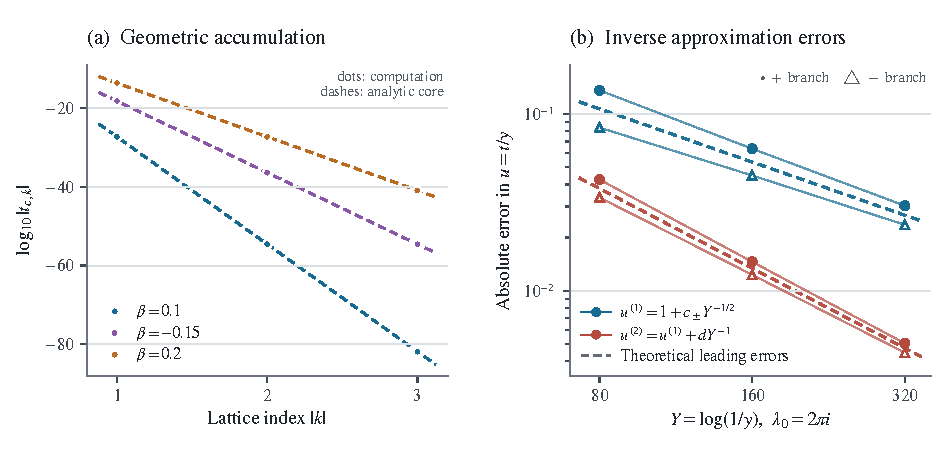
\includegraphics[width=\textwidth]{figures/complex_resonance_figure.pdf}
\caption{Complex resonance and inverse branching.
\textup{(a)} Recorded critical points for
$\eps=i\beta$, $\beta\in\{0.1,-0.15,0.2\}$, $|k|=1,2,3$.
The dashed lines are
$\log_{10}|a(i\beta,0)|-2\pi|k|/(|\beta|\log10)$; the discrepancies
are too small to resolve at this scale.
\textup{(b)} Absolute errors in $u_\pm=t_\pm/y$ for
$\eps=2\pi i/Y$, $Y=80,160,320$. Circles and triangles distinguish
the two branches. First and second approximations retain terms
through $Y^{-1/2}$ and $Y^{-1}$, respectively. The reference curves
$|d|Y^{-1}$ and $|e_\pm|Y^{-3/2}$ use the exact coefficients derived
in \cref{app:figure-coefficient}; none is fitted to the data.}
\label{fig:complex-resonance}
\end{figure}

All these numerical figures are diagnostics, not interval
certificates. The small residual of an equation near a critical
point is not by itself a rigorous root-error bound. Furthermore,
direct subtraction of the two order-one terms in the endpoint
defect loses digits when $y=e^{-Y}$ is extremely small; the paired
normal form avoids that subtraction. Preliminary differentiation
of a generic numerical polylogarithm routine precisely at integer
order was also less reliable than the defining-series and
logistic-integral routes. The verification programs therefore keep
those routes explicit.

\subsection{Reproducibility and repository integration}

The source package contains one complete article source, its PDF,
the vector figure and plotting program, the four verification
programs, their JSON records, a dependency file, a build command,
and a manifest of checksums. All mathematical arguments are in the
article; running Python is not necessary to follow a proof. Running
the programs is useful for reproducing the finite diagnostics.

The integration notes propose one canonical article location and
cross-links from both programmes. They preserve the predecessor
reports and distinguish a theorem extension from an erratum.
No repository file was edited as part of this report. The supplied
package is intended for review and subsequent integration.


\section{Further research questions and a proposed programme}
\label{sec:questions}

The questions below are not assertions of results established here.
They are selected to use the exact formulas while addressing
limitations that remain after the local existence and coefficient
calculations have been completed.

\subsection{Certified domains and the geometry of inverse coefficients}

\paragraph{Q1. Obtain effective convergence domains.}
For actual tails $R_{p,q,a}$, determine explicit polydiscs and
computable constants for \eqref{eq:geometric-inverse}, the critical
charts $a,b$, and the split charts $W_\pm$. A practical starting
point is the factorial majorant in \cref{thm:sector}, followed by
an explicit contraction or interval Newton estimate for the
implicit equation. A useful deliverable would accept $p,q,a$,
a target precision, and a sector, and return both an approximation
and a certified error. The main difficulty is retaining useful
bounds near a fold, where an ordinary inverse condition number
diverges and the quadratic coordinate must be used instead.

\paragraph{Q2. Determine large coefficient-index asymptotics.}
The exact pole order of $v_n(\eta)$ as a function of $\eta$ is known
from \cref{thm:sharp-poles}. What is the asymptotic behavior of
$v_n(\eta)$ as $n\to\infty$ at a fixed admissible $\eta$?
For a given polylogarithm tail, locate the dominant solutions of
the coupled equations
\[
 H(T,\eta,V)=0,\qquad H_V(T,\eta,V)=0,
\]
where $H$ is the left side of \eqref{eq:chart-model} minus $1$.
Decide when a simple quadratic singularity supplies an
$n^{-3/2}$ coefficient factor, which competing singularities have
the same modulus, and how the answer changes as $\eta$ approaches
$p/q$. This would connect the Catalan pole law with actual
convergence radii, without identifying those two different questions
prematurely.

\paragraph{Q3. Classify arithmetic cancellations and missing sectors.}
For finitely many shifts $a_\nu$ and weights $w_\nu$, consider
$\sum_\nu w_\nu\cY_{p,q,a_\nu}$. The first $h$ analytic tail
coefficients vanish precisely when the explicit zeta-derivative
expressions in \eqref{eq:Rcoeff} satisfy $h$ linear relations.
Classify cancellations that persist for infinitely many coefficient
indices, especially for rational shifts or roots-of-unity
combinations. The half-shift parity at $q=1$ is an elementary
example; differentiation in the order generally removes those
zeros. Determine which distribution identities preserve a
nontrivial support restriction for $q\ge2$, and what restrictions
remain after compositional inversion.

\subsection{Complex-order critical values and global inverse structure}

\paragraph{Q4. Extend the critical classification beyond small imaginary order.}
The local critical lattice is now exhausted for sufficiently small
fixed $\beta\ne0$. For larger $\beta$, the constant-term balance
suggests the limiting argument
\[
 \theta_\beta=-\frac1\beta
   \log\left|\frac{i\beta\,\zeta(1+i\beta)}
                     {\Gamma(1-i\beta)}\right|.
\]
Determine a complete principal-sheet criterion in terms of this
quantity and the analytic tail, including the boundary cases
$\theta_\beta=\pm\pi$. Establish how the lattice enters or leaves
a chosen logarithm sheet, and quantify its critical-value
asymptotics uniformly in the remaining parameter ranges.
A statement on the logarithmic cover must be distinguished from
one on a fixed principal sheet.

\paragraph{Q5. Describe which inverse sheets meet at the accumulating values.}
The local square-root branch values of $F_{i\beta}^{-1}$ accumulate
at zero. Which of them are accessible from a particular inverse
germ by continuation along specified paths? What is the monodromy
action on that connected family of inverse sheets? Can a
description of the complete local lattice be converted into
precise boundary behavior for an inverse branch on a slit or
spiraling domain? Accumulation of branch values alone does not
answer whether a chosen inverse has a natural boundary, and that
global inference remains to be proved or disproved.

\paragraph{Q6. Classify higher-multiplicity inverse resonances.}
Replace the dilogarithm defect by a higher Taylor-subtracted
remainder, a normalized order jet, or a finite linear combination
of such jets. Determine which parameter choices make the limiting
inverse equation have multiplicity $m>2$. A proved classification
should identify the minimal unfolding parameters, the analogue of
the exact branch curve in \eqref{cx:lambda-critical}, and the
fractional inverse-logarithmic scale forced by the multiplicity.
The natural procedure is to compute the limiting logarithmic
polynomial exactly before applying a Weierstrass or Newton-polygon
analysis. It is not enough to infer an $m$th-root scale from a
numerical collision of approximate roots.

\subsection{Uniform resurgence and nonlinear reconstruction}

\paragraph{Q7. Match the revived coefficient crossover with optimal truncation.}
Proposition~\ref{prop:coefficient-crossover} already resolves the
coefficient-level double limit with
$\eps\log k$ bounded. Develop a function-level expansion uniform
when $x\to\infty$, $s\to N$, and $\eps\log x$ remains bounded.
It should interpolate between the terminating integer-order
polynomial, the factorially divergent order jet, and the exact
exponential completion. The next step is to prove an explicit
remainder for a truncation index proportional to $x$, and then
carry that estimate through the nonlinear inverse. The exact
gamma-product formula and the paired Borel integral give two
independent starting points for this analysis.

\paragraph{Q8. Derive Lerch and cyclotomic analogues of the residue kernel.}
For periodically weighted Dirichlet series, identify the analogue
of
$\pi\xi/\sin(\pi\xi)$ in \eqref{eq:borel-KN}. Determine its poles,
the rays on which they lie, the coefficients recovered by the
first order jet, and the effect of shift differentiation.
For root-of-unity weights one expects finite combinations of
elementary trigonometric kernels, but the precise branch factors
and the correct physical completion must be derived. The goal
is an exact formula with a specified lateral convention and
domain, followed by a nonlinear inverse application.

\paragraph{Q9. Compute noninteger inverse Stokes transformations.}
At integer order \eqref{eq:borel-inverse-coeff} gives every
exponential inverse sector through finite composition sums.
For noninteger order, determine the discontinuity of a specified
sectorial compositional inverse from the exact discontinuity
\eqref{eq:borel-disc}. Relate its first derivative in the order
to the integer residue formula, while controlling the deformation
of the algebraic core. This would test how much of the triangular
reconstruction survives a nonlinear change of dependent variable.

\paragraph{Q10. Establish uniform complex-argument Borel formulas.}
The exact lateral identities here are proved for real $x>0$.
Continue them to complex sectors with explicit compatible
polylogarithm branches and quantitative bounds as a summation
ray approaches a pole direction. Determine the connection
formulas when the Laplace contour must rotate across several
rays. The integral representation suggests the extension, but
the contour deformation, the argument of $x^{s+1}$, and the
reflected polylogarithm must be tracked together.

\subsection{Recommended order of work}

For repository development, the most direct next project is Q1:
it turns the convergent charts into certified evaluators and
supplies sharper test cases for the other questions. Q2 and Q4
then address the actual singularity geometry. Q7 and Q9 are the
most substantial asymptotic continuation of the present order-jet
idea. Q3 and Q8 provide the strongest connection to the arithmetic
side of the polylogarithm programme.

Before a publication-priority claim, carry out a dedicated comparison
with the full original literature on complex polylogarithm zeros,
near-integer order evaluation, and complete Fermi--Dirac expansions.
The proof status of the formulas in this report and the priority
status of their presentation are separate matters.


\appendix
\section{The coefficient behind the numerical error reference}
\label{app:figure-coefficient}

Write $\lambda=2\pi i$, $r_1=\gamma-1$, and
\[
 r_2=\frac{r_1^2+\zeta(2)+1}{2},\qquad
 r_3=\frac{r_1^3}{6}+\frac{r_1(\zeta(2)+1)}{2}
       +\frac{\zeta(3)-1}{3},\qquad
 D=r_2+\gamma_1,\qquad J=\frac{\gamma_2}{2}-r_3.
\]
Here $\zeta(1+w)=w^{-1}+\gamma-\gamma_1w+\gamma_2w^2/2+\cdots$.
For the two local branches, choose
$c_\pm=\pm\sqrt{-2\lambda D}$, with the principal square root for $c_+$.
The next coefficient after
$d=-\lambda(r_1+4D/3)$ is
\[
 e_\pm=\frac{\lambda^2}{c_\pm}
 \left(J+\frac{r_1^2}{2}+(3\gamma-2)D+\frac{13D^2}{9}\right).
\]
Thus
\[
 \frac{t_\pm}{y}
 =1+\frac{c_\pm}{\sqrt Y}+\frac dY+
       \frac{e_\pm}{Y^{3/2}}+O(Y^{-2}).
\]
To verify the formula directly, set $x=Y^{-1}$, $u=1+w$ and expand
the exact paired equation, omitting its exponentially small analytic
remainder:
\[
 \begin{split}
 0={}&-\frac{w^2}{2}+\frac{w^3}{6}-\frac{w^4}{12}
 -\lambda x\left(D+(D+r_1)w+\frac{\gamma w^2}{2}\right)
 +\lambda^2Jx^2\\
 &\quad+O(w^5+xw^3+x^2w+x^3)+O(e^{-Y}).
 \end{split}
\]
The coefficients of $x$, $x^{3/2}$ and $x^2$ give $c_\pm$, $d$ and
$e_\pm$ in that order. The analytic square-root chart justifies this
coefficient calculation and its remainder. The reference curves in
panel~\textup{(b)} are therefore $|d|/Y$ and $|e_\pm|/Y^{3/2}$, where
\[
 |d|\simeq 8.561352970598396,\qquad
 |e_+|=|e_-|\simeq 27.13447947885805.
\]

\section{Literature-search boundaries}
\label{app:literature}
The primary mathematical inputs used for the proofs were inspected
in full at the relevant formulas or sections. They include the
DLMF local expansions, the predecessor repository proofs, the
near-integer computational formulas, and the full author manuscript
of Gil--Segura--Temme. The bibliography supplies stable locations
rather than relying on search-result snippets for those inputs.

There is classical precedent for oscillatory boundary accumulation.
Gawronski and Stadtm\"uller \cite{gawronski-stadtmuller} exhibit
infinitely many zeros in $(0,1)$ for the series
$\sum_{n\ge0}\sin(\log(n+1))z^n$. This is a combination of
complex-order polylogarithms rather than the single-polylogarithm
family studied here. It is a reason to regard the explicit common
charts, critical values, and inverse unfolding as the relevant
increments, rather than claiming a new general mechanism for
boundary accumulation.

The search also identified sources requiring fuller comparison before
a claim of publication priority. Fornberg--K\"olbig's
\emph{Complex zeros of the Jonquière or polylogarithm function}
\cite{fornberg-kolbig} and Paulsen's \emph{The Behavior of
Polylogarithms at $z=1$} \cite{paulsen} were located through primary
bibliographic records and available descriptions, but their full texts
were not obtained in this review. Gawronski's 1979 paper
\cite{gawronski} likewise requires inspection of the original
hypotheses. These access limits do not enter any proof in the article.
They do limit what the review can say about the historical priority of
the local zero-lattice mechanism.

The most appropriate present description is therefore a proved
research report containing explicit extensions, a coherent order-jet
framework, and precisely scoped corrections. The contribution claims
refer to the formulas and arguments actually established here.


\begin{thebibliography}{99}
\small\raggedright
\setlength{\itemsep}{5pt}

\bibitem{repo-resonance}
ProveIt repository,
\emph{Resonance continuation: uniform resonance and Stieltjes finite
parts; research question R1}.
The report in
\texttt{resonance-correlations-nonseparable-jets}, especially
\texttt{sections/02\_resonance.tex} and
\texttt{sections/07\_questions.tex}.
Snapshot \snapshot.
\href{https://github.com/VladimirReshetnikov/ProveIt/blob/9ec0f0406afe7a5475b03ff65ed91f7e283979b8/Analysis/Polylogarithms/docs/reports/uniform-transition-continuation/continuations/resonance-correlations-nonseparable-jets/sections/02_resonance.tex}{Pinned theorem source};
\href{https://github.com/VladimirReshetnikov/ProveIt/blob/9ec0f0406afe7a5475b03ff65ed91f7e283979b8/Analysis/Polylogarithms/docs/reports/uniform-transition-continuation/continuations/resonance-correlations-nonseparable-jets/sections/07_questions.tex}{pinned questions}.

\bibitem{repo-lambert}
ProveIt repository,
\emph{Logarithmic Critical Endpoint Lambert Charts},
\texttt{article.tex}, Theorem \texttt{thm:lambert}.
Snapshot \snapshot.
\href{https://github.com/VladimirReshetnikov/ProveIt/blob/9ec0f0406afe7a5475b03ff65ed91f7e283979b8/Analysis/Transseries/docs/series-and-transseries/Logarithmic_Critical_Endpoint_Lambert_Charts/article.tex}{Pinned source}.

\bibitem{repo-confluent}
ProveIt repository,
\emph{Confluent Critical Transseries at the Exponent-Two Boundary},
\texttt{Confluent\_Critical\_Transseries.tex}.
Snapshot \snapshot.
\href{https://github.com/VladimirReshetnikov/ProveIt/blob/9ec0f0406afe7a5475b03ff65ed91f7e283979b8/Analysis/Transseries/docs/series-and-transseries/Confluent_Critical_Transseries_Exponent_Two_Boundary/Confluent_Critical_Transseries.tex}{Pinned source}.

\bibitem{dlmf-poly}
NIST Digital Library of Mathematical Functions,
\S25.12, \emph{Polylogarithms}, especially
(25.12.10)--(25.12.16).
\url{https://dlmf.nist.gov/25.12}.
Consulted 12 October 2026.

\bibitem{dlmf-lerch}
NIST Digital Library of Mathematical Functions,
\S25.14, \emph{Lerch's Transcendent}, especially
(25.14.3\_1)--(25.14.3\_2).
\url{https://dlmf.nist.gov/25.14}.
Consulted 12 October 2026.

\bibitem{dlmf-hurwitz}
NIST Digital Library of Mathematical Functions,
\S25.11, \emph{Hurwitz Zeta Function}, especially
the Hermite integral (25.11.29).
\url{https://dlmf.nist.gov/25.11}.
Consulted 12 October 2026.

\bibitem{dlmf-gamma}
NIST Digital Library of Mathematical Functions,
\S5.11, \emph{Asymptotic Expansions}, including Gamma-function ratios.
\url{https://dlmf.nist.gov/5.11}.
Consulted 12 October 2026.

\bibitem{roughan}
M. Roughan,
\emph{The Polylogarithm Function in Julia},
arXiv:2010.09860 (2020), especially \S4.3.
\url{https://arxiv.org/abs/2010.09860}.

\bibitem{bailey-borwein}
D.~H. Bailey and J.~M. Borwein,
Crandall's computation of the incomplete Gamma function and the
Hurwitz Zeta function, with applications to Dirichlet $L$-series,
\emph{Applied Mathematics and Computation}
\textbf{268} (2015), 462--477.
\href{https://doi.org/10.1016/j.amc.2015.06.048}
{doi:10.1016/j.amc.2015.06.048}.
\href{https://www.davidhbailey.com/dhbpapers/lerch.pdf}
{Author manuscript}.

\bibitem{flajolet-sedgewick}
P. Flajolet and R. Sedgewick,
\emph{Analytic Combinatorics},
Cambridge University Press, 2009.
\url{https://algo.inria.fr/flajolet/Publications/book.pdf}.

\bibitem{gessel}
I.~M. Gessel,
\emph{Lagrange Inversion},
arXiv:1609.05988 (2016).
\url{https://arxiv.org/abs/1609.05988}.

\bibitem{corless}
R.~M. Corless, G.~H. Gonnet, D.~E.~G. Hare, D.~J. Jeffrey,
and D.~E. Knuth,
On the Lambert $W$ function,
\emph{Advances in Computational Mathematics}
\textbf{5} (1996), 329--359.
\href{https://doi.org/10.1007/BF02124750}
{doi:10.1007/BF02124750}.

\bibitem{kalugin}
G.~A. Kalugin and D.~J. Jeffrey,
\emph{Convergence in $\C$ of series for the Lambert $W$ function},
arXiv:1208.0754 (2012).
\url{https://arxiv.org/abs/1208.0754}.

\bibitem{costin}
O. Costin and S. Garoufalidis,
\emph{Resurgence of the fractional polylogarithms},
arXiv:math/0701743, version 4 (2009).
\url{https://arxiv.org/abs/math/0701743}.

\bibitem{dingle}
R.~B. Dingle,
The Fermi--Dirac integrals
$\mathcal F_p(\eta)
=(p!)^{-1}\int_0^\infty
\varepsilon^p(e^{\varepsilon-\eta}+1)^{-1}\,d\varepsilon$,
\emph{Applied Scientific Research, Section B}
\textbf{6} (1957), 225--239.
\href{https://doi.org/10.1007/BF02920379}
{doi:10.1007/BF02920379}.

\bibitem{garoni}
T.~M. Garoni, N.~E. Frankel, and M.~L. Glasser,
Complete asymptotic expansions of the Fermi--Dirac integrals,
\emph{Journal of Mathematical Physics}
\textbf{42}, no.~4 (2001), 1860--1868.
\href{https://doi.org/10.1063/1.1350634}
{doi:10.1063/1.1350634}.

\bibitem{gil}
A. Gil, J. Segura, and N.~M. Temme,
Complete asymptotic expansions for the relativistic Fermi--Dirac integral,
\emph{Applied Mathematics and Computation}
\textbf{412} (2022), article 126618.
\href{https://doi.org/10.1016/j.amc.2021.126618}
{doi:10.1016/j.amc.2021.126618}.
\href{https://arxiv.org/abs/2108.11210}
{arXiv:2108.11210}, version 2 consulted.

\bibitem{vepstas}
L. Vepstas,
\emph{The Polylog and the Riemann Hypothesis},
author draft, 29 October 2023, especially pp.~3--5.
\url{https://linas.org/math/polylog.pdf}.
Consulted for the specifically discussed modulus and accumulation claims.

\bibitem{osullivan}
C. O'Sullivan,
Zeros of the dilogarithm,
\emph{Mathematics of Computation}
\textbf{85}, no.~302 (2016), 2967--2993.
\href{https://doi.org/10.1090/mcom/3065}{doi:10.1090/mcom/3065}.
\href{https://fsw01.bcc.cuny.edu/cormac.osullivan/Research/dilog_zeros_final.pdf}
{Author-hosted version}, especially \S8.1.
The \href{https://fsw01.bcc.cuny.edu/cormac.osullivan/Research/research.htm}
{author's research page} identifies this text with the published paper.

\bibitem{gawronski}
W. Gawronski,
On the zeros of power series with rational coefficients III,
\emph{Archiv der Mathematik}
\textbf{32}, no.~4 (1979), 368--376.
\href{https://doi.org/10.1007/BF01238513}
{doi:10.1007/BF01238513}.
Bibliographic record verified; full theorem hypotheses not inspected.

\bibitem{gawronski-stadtmuller}
W. Gawronski and U. Stadtm\"uller,
On the zeros of power series with exponential logarithmic coefficients,
\emph{Canadian Mathematical Bulletin}
\textbf{24}, no.~3 (1981), 257--271.
\href{https://doi.org/10.4153/CMB-1981-042-1}
{doi:10.4153/CMB-1981-042-1}.

\bibitem{fornberg-kolbig}
B. Fornberg and K.~S. K\"olbig,
Complex zeros of the Jonquière or polylogarithm function,
\emph{Mathematics of Computation}
\textbf{29}, no.~130 (1975), 582--599.
\href{https://doi.org/10.1090/S0025-5718-1975-0369278-0}
{doi:10.1090/S0025-5718-1975-0369278-0}.
Full text not obtained in this review.

\bibitem{paulsen}
W. Paulsen,
The Behavior of Polylogarithms at $z=1$,
\emph{Complex Variables, Theory and Application}
\textbf{47}, no.~9 (2002), 815--819.
\href{https://doi.org/10.1080/02781070290032199}
{doi:10.1080/02781070290032199}.
Publisher description consulted; full text not obtained.

\end{thebibliography}
\end{document}
